\documentclass[11pt]{article}

% Language setting
\usepackage[spanish]{babel}

% Page size and margins
\usepackage[a4paper,top=2cm,bottom=2cm,left=3cm,right=3cm,marginparwidth=1.75cm]{geometry}

% Useful packages
\usepackage{amsmath}
\usepackage{graphicx}
\usepackage{tikz}
\usetikzlibrary{arrows.meta,positioning,fit,backgrounds,calc,babel}
\usepackage{hyperref}
\usepackage{setspace}
\usepackage{tocloft}
\usepackage{listings}

\hypersetup{
  colorlinks = true,
  citecolor = blue,
  urlcolor = blue,
  linkcolor=[rgb]{0,0,1}
}

\lstset{
  basicstyle=\ttfamily\small,   % monospace
  numbers=left,                 % line numbers
  numberstyle=\ttfamily\small,  % line number font
  stepnumber=1,                 % every line numbered
  numbersep=10pt,               % gap between numbers and code
  xleftmargin=2em,              % left indent for numbers
  showstringspaces=true,
  keepspaces=true,
  columns=fullflexible
}

\begin{document}

% Title page
\begin{titlepage}
    \centering

    % Replace with your UC logo file
    
\includegraphics{resources/uc_logo.png}

    \vspace{2cm}

    {\Large\bfseries\itshape
    Facultad\\
    de Ciencias\\
    }

    \vspace{2cm}

    {\LARGE\bfseries
    Enriquecimiento automático\\
    de las revisiones de código\\
    en proyectos software con\\
    desarrollo dirigido por modelos\\
    }

    \vspace{1cm}

    {\LARGE\bfseries\itshape
    Automatic Enrichment of Code Reviews\\
    in Model-Driven Software Development Projects\\
    }

    \vspace{2cm}

    {\Large\bfseries
    Trabajo de Fin de Grado\\
    para acceder al
    \par}

    \vspace{0.5cm}

    {\Large\bfseries GRADO EN INGENIERÍA INFORMÁTICA\par}

    \vfill

    \begin{flushright}
        {\fontsize{14}{16.8}\selectfont\bfseries Autor: Samuel Díaz Aja\par}
        \vspace{0.25cm}
        {\fontsize{14}{16.8}\selectfont\bfseries Director: Alfonso de la Vega Ruiz\par}
        \vspace{0.25cm}
        {\fontsize{14}{16.8}\selectfont\bfseries Co-Director: Pablo Sánchez Barreiro\par}
        \vspace{1cm}
        {\large\bfseries Junio - 2026\par}
    \end{flushright}
\end{titlepage}

\onehalfspacing
\renewcommand{\cftsecleader}{\cftdotfill{\cftdotsep}}

\newpage
\null
\thispagestyle{empty}
\newpage

\tableofcontents
\listoffigures

\newpage

\phantomsection
\addcontentsline{toc}{section}{Resumen}
\begin{abstract}
Este trabajo presenta RAMA (\textit{pull/change Request Augmentation for Model Awareness}), una herramienta de apoyo a la revisión de cambios en proyectos de Ingeniería del software Dirigida por Modelos o \textit{Model-Driven Software Engineering (MDSE)}. RAMA se plantea como un bot de revisión consciente de modelos para proyectos basados en MDSE; no sustituye al sistema de revisión existente, sino que lo complementa con información específica sobre los artefactos de modelado.

RAMA se integra en el flujo habitual de desarrollo de proyectos que utilizan git como sistema de control de versiones, y que se encuentren alojados en GitHub. Utilizando procesos automatizados  mediante GitHub Actions, analiza los cambios realizados en archivos de modelo y metamodelo dentro de las \textit{pull requests}. A continuación, complementa el \texttt{diff} textual tradicional con información a nivel de modelo.

La herramienta detecta los archivos relevantes modificados en una \textit{pull request}, recupera las versiones relevantes del modelo de las ramas del repositorio, y realiza una comparación a nivel de modelo con la herramienta especializada EMF Compare. El punto central del enfoque es separar dos responsabilidades: GitHub indica qué archivos han cambiado, mientras que EMF Compare permite determinar qué ha cambiado dentro de los modelos y si esas modificaciones son significativas desde el punto de vista estructural. Posteriormente, RAMA transforma los resultados a informes textuales y gráficos, y publica dichos informes como un comentario en la \textit{pull request} analizada. De esta forma, RAMA introduce conciencia de modelos en el proceso de revisión de código y reduce el esfuerzo necesario para interpretar modificaciones en artefactos de modelado.

La versión actual de RAMA incluye la funcionalidad necesaria para detectar cambios en modelos y metamodelos, así como posibles conflictos derivados del desarrollo colaborativo. La herramienta se encuentra públicamente disponible en un repositorio de código abierto, y este trabajo incluye instrucciones para su configuración y utilización en proyectos MDSE existentes. Además, cuenta con pruebas automatizadas y una batería de casos de comparación orientadas a verificar su correcto funcionamiento.
\end{abstract}

\phantomsection
\addcontentsline{toc}{section}{Palabras clave}
\section*{Palabras clave}

\textit{Ingeniería del Software Dirigida por Modelos, Eclipse Modeling Framework, Ecore, Revisión de Código, Pull Requests, Visualización de Modelos, Comparación de Modelos, EMF Compare, GitHub Actions}

\newpage

\phantomsection
\addcontentsline{toc}{section}{\textit{Abstract}}
\renewcommand{\abstractname}{Abstract}
\begin{abstract}
This work presents RAMA (\textit{pull/change Request Augmentation for Model Awareness}), a tool designed to support the review of changes in \textit{Model-Driven Software Engineering} (MDSE) projects. RAMA is conceived as a model-aware review bot for MDSE-based projects. Rather than replacing the existing code review process, it complements it by providing information specific to modeling artifacts.

RAMA integrates into the standard development workflow of projects that use Git as their version control system and are hosted on GitHub. It analyzes changes made to model and metamodel files within \textit{pull requests} through automated workflows implemented with GitHub Actions. It then augments the traditional textual \texttt{diff} with model-level information.

The tool identifies the relevant files modified in a \textit{pull request}, retrieves the corresponding versions of the models from the repository branches, and performs a model-level comparison using the specialized EMF Compare framework. The core idea of the approach is to separate two responsibilities: GitHub determines which files have changed, while EMF Compare identifies what has changed within the models and whether those modifications are structurally significant. RAMA subsequently transforms the comparison results into textual and graphical reports, which are published as a comment on the analyzed \textit{pull request}. In this way, RAMA introduces model awareness into the code review process and reduces the effort required to interpret changes in modeling artifacts.

The current version of RAMA provides the functionality required to detect changes in models and metamodels, as well as potential conflicts arising from collaborative development. The tool is publicly available as an open-source project, and this work includes instructions for its configuration and use in existing MDSE projects. In addition, RAMA is supported by automated tests and a comprehensive comparison test suite to verify its correct operation.
\end{abstract}
\renewcommand{\abstractname}{Resumen}


\phantomsection
\addcontentsline{toc}{section}{\textit{Keywords}}
\section*{Keywords}

\textit{Model-Driven Software Engineering, Eclipse Modeling Framework, Ecore, Code Review, Pull Requests, Model Visualization, Model Comparison, EMF Compare, GitHub Actions}

\newpage

\phantomsection
\addcontentsline{toc}{section}{Acrónimos}
\section*{Acrónimos}

\begin{tabular}{ll}
API & \textit{Application Programming Interface} \\
EMF & \textit{Eclipse Modeling Framework} \\
HTML & \textit{HyperText Markup Language} \\
JAR & \textit{Java Archive} \\
JSON & \textit{JavaScript Object Notation} \\
MDSE & \textit{Model-Driven Software Engineering} \\
PR & \textit{Pull Request} \\
RAMA & \textit{pull/change Request Augmentation for Model Awareness} \\
SVG & \textit{Scalable Vector Graphics} \\
UML & \textit{Unified Modeling Language} \\
URI & \textit{Uniform Resource Identifier} \\
URL & \textit{Uniform Resource Locator} \\
UTF-8 & \textit{Unicode Transformation Format, 8-bit} \\
XML & \textit{Extensible Markup Language} \\
XMI & \textit{XML Metadata Interchange} \\
\end{tabular}

\newpage

\section{Introducción}

Los sistemas de control de versiones son una pieza central en la gestión de la evolución del código fuente, ya que permiten registrar de forma ordenada los cambios realizados sobre un proyecto, recuperar estados anteriores y coordinar el trabajo de varios desarrolladores. En este contexto, el historial del repositorio puede entenderse como un árbol de versiones, donde cada \textit{commit} representa un estado del código y las ramas permiten desarrollar funcionalidades, corregir errores o experimentar con cambios de forma paralela sin afectar directamente a la línea principal de desarrollo.

Para integrar estos cambios en la rama principal se emplean habitualmente las \textit{pull requests}, que actúan como un mecanismo de propuesta, discusión y validación antes de incorporar nuevo código. Durante este proceso, otros desarrolladores pueden revisar las modificaciones, detectar posibles errores, sugerir mejoras y dejar comentarios sobre partes concretas del código, convirtiendo la revisión en una práctica fundamental para mantener la calidad, la trazabilidad y la coherencia del proyecto.

En los procesos actuales de desarrollo de software, la revisión de cambios y el control de versiones suele apoyarse en plataformas colaborativas como GitHub. Estas plataformas presentan las modificaciones de una \textit{pull request} principalmente como diferencias textuales entre archivos. Este mecanismo es eficaz para código fuente, documentación o configuración, pero resulta limitado cuando los archivos modificados no poseen un formato textual legible. Este es el caso en los modelos y metamodelos utilizados en \textit{Model-Driven Software Engineering (MDSE)}, siendo esta la motivación para realizar este proyecto.

\subsection{Contexto}

El contexto técnico de este trabajo se sitúa en la Ingeniería del software Dirigida por Modelos. En este enfoque, los modelos se utilizan como representaciones de alto nivel de sistemas, dominios o lenguajes específicos, de forma que el desarrollo no se apoya únicamente en código fuente, sino también en artefactos que describen estructura, comportamiento, restricciones o conceptos del dominio. Estos modelos son útiles precisamente porque permiten trabajar con abstracciones más cercanas al problema que se quiere resolver.

Junto a los modelos aparecen también los metamodelos, que definen la estructura que deben seguir dichos modelos: qué tipos de elementos pueden existir, qué atributos tienen y qué relaciones pueden establecerse entre ellos. Por ello, en un proyecto basado en MDSE no solo evolucionan los modelos concretos del sistema, sino también los lenguajes o esquemas que les dan forma.

Para que esas abstracciones sean manejables, los modelos suelen requerir herramientas específicas de edición, visualización, validación y transformación. Aunque se almacenen en ficheros dentro de un repositorio, ese almacenamiento responde principalmente a una necesidad de persistencia e intercambio entre herramientas. El fichero serializado no es, en general, la representación pensada para que una persona lo lea o lo manipule directamente: puede contener identificadores, referencias internas, elementos anidados y detalles propios del formato de persistencia que dificultan la interpretación manual.

En el ecosistema EMF, por ejemplo, los modelos y metamodelos se almacenan habitualmente en formatos basados en XML o XMI \cite{XMI}. EMF proporciona una infraestructura ampliamente utilizada para definir metamodelos, cargar modelos y manipularlos como objetos \cite{emf-book,emf-docs}. Sirius permite construir entornos gráficos de modelado específicos de dominio \cite{sirius-docs}. Epsilon reúne lenguajes y herramientas para tareas habituales sobre modelos, como validación, transformación, generación de código, comparación, mezcla o visualización \cite{epsilon-docs}. EMF Compare ofrece soporte genérico para comparar y mezclar modelos conformes a distintos metamodelos \cite{emfcompare-overview}. Estas herramientas muestran que MDSE cuenta con soporte maduro para crear, editar, transformar y comparar modelos.

El problema aparece cuando estos artefactos se integran en los flujos habituales de control de versiones. En la práctica, muchos proyectos almacenan modelos EMF en repositorios Git junto con el código fuente y los revisan mediante plataformas generalistas como GitHub. En ese escenario aparece una distancia entre las herramientas de modelado y el flujo cotidiano de revisión: GitHub muestra diferencias textuales sobre los archivos serializados, mientras que el significado real del cambio pertenece al nivel del modelo. Esta representación textual no siempre refleja de forma clara el cambio conceptual realizado: una modificación pequeña en el modelo puede generar muchas líneas cambiadas, mientras que un cambio estructural importante puede quedar repartido entre fragmentos difíciles de interpretar. El Listado~\ref{lst:modelo-xmi} muestra un ejemplo de esta serialización en XMI, que ilustra la dificultad de revisar modelos únicamente a partir de su contenido textual.

\begin{lstlisting}[caption={Ejemplo de modelo Ecore serializado en XMI.},label={lst:modelo-xmi},basicstyle=\ttfamily\scriptsize]
<?xml version="1.0" encoding="UTF-8"?>
<ecore:EPackage xmi:version="2.0" xmlns:xmi="http://www.omg.org/XMI"
  xmlns:xsi="http://www.w3.org/2001/XMLSchema-instance"
  xmlns:ecore="http://www.eclipse.org/emf/2002/Ecore"
  name="library" nsURI="library" nsPrefix="">
    <eClassifiers xsi:type="ecore:EClass" name="Library">
      <eStructuralFeatures xsi:type="ecore:EReference" name="writers"
        upperBound="-1" eType="#//Writer" containment="true"/>
      <eStructuralFeatures xsi:type="ecore:EReference" name="books"
        upperBound="-1" eType="#//Book" containment="true"/>
      <eStructuralFeatures xsi:type="ecore:EReference" name="publishers"
        upperBound="-1" eType="#//Publisher" containment="true"/>
      <eStructuralFeatures xsi:type="ecore:EReference" name="members"
        upperBound="-1" eType="#//Member" containment="true"/>
    </eClassifiers>
    <eClassifiers xsi:type="ecore:EClass" name="Writer">
      <eStructuralFeatures xsi:type="ecore:EAttribute" name="name"
        eType="ecore:EDataType http://www.eclipse.org/emf/2002/Ecore#//EString"/>
      <eStructuralFeatures xsi:type="ecore:EReference" name="books"
        upperBound="-1" eType="#//Book"/>
    </eClassifiers>
    <eClassifiers xsi:type="ecore:EClass" name="Book">
      <eStructuralFeatures xsi:type="ecore:EAttribute" name="title"
        eType="ecore:EDataType http://www.eclipse.org/emf/2002/Ecore#//EString"/>
      <eStructuralFeatures xsi:type="ecore:EAttribute" name="pages"
        eType="ecore:EDataType http://www.eclipse.org/emf/2002/Ecore#//EInt"
        defaultValueLiteral="100"/>
      <eStructuralFeatures xsi:type="ecore:EAttribute" name="yearOfPublication"
        eType="ecore:EDataType http://www.eclipse.org/emf/2002/Ecore#//EInt"/>
      <eStructuralFeatures xsi:type="ecore:EAttribute" name="category"
        eType="#//BookCategory"/>
      <eStructuralFeatures xsi:type="ecore:EReference" name="publisher"
        eType="#//Publisher"/>
    </eClassifiers>
    <eClassifiers xsi:type="ecore:EClass" name="Publisher">
      <eStructuralFeatures xsi:type="ecore:EAttribute" name="name"
        eType="ecore:EDataType http://www.eclipse.org/emf/2002/Ecore#//EString"/>
      <eStructuralFeatures xsi:type="ecore:EAttribute" name="country"
        eType="ecore:EDataType http://www.eclipse.org/emf/2002/Ecore#//EString"/>
    </eClassifiers>
    <eClassifiers xsi:type="ecore:EClass" name="Member">
      <eStructuralFeatures xsi:type="ecore:EAttribute" name="name"
        eType="ecore:EDataType http://www.eclipse.org/emf/2002/Ecore#//EString"/>
      <eStructuralFeatures xsi:type="ecore:EAttribute" name="membershipId"
        eType="ecore:EDataType http://www.eclipse.org/emf/2002/Ecore#//EInt"/>
      <eStructuralFeatures xsi:type="ecore:EReference" name="borrowedBooks"
        upperBound="-1" eType="#//Book"/>
    </eClassifiers>
    <eClassifiers xsi:type="ecore:EEnum" name="BookCategory">
      <eLiterals name="History"/>
      <eLiterals name="Geography" value="1"/>
    </eClassifiers>
</ecore:EPackage>
\end{lstlisting}

\subsection{Marco de investigación}

Este trabajo se relaciona con líneas de investigación existentes en el Grupo de Ingeniería del Software y Tiempo Real (ISTR) del Departamento de Ingeniería Informática y Electrónica de la Universidad de Cantabria, especialmente con aquellas orientadas a la Ingeniería del software Dirigida por Modelos, la evolución de modelos y el soporte a tareas de análisis, comparación y revisión. Dentro de este contexto se sitúan trabajos como Peacemaker, una herramienta para resolver conflictos en modelos XMI aprovechando la información marcada por los sistemas de control de versiones \cite{peacemaker}; Picto Diff, una extensión de Epsilon Picto para revisar visualmente cambios en modelos \cite{picto,picto-diff}; y Munidiff, que propone representaciones textuales y gráficas de diferencias entre modelos, y es la herramienta que se ha utilizado en este trabajo para renderizar dichas representaciones \cite{munidiff,munidiff-paper}. Estas contribuciones proporcionan el marco de investigación sobre el que se plantea la integración de información a nivel de modelo en flujos colaborativos de desarrollo.

RAMA se sitúa dentro de esta evolución, abordando un punto concreto del flujo de desarrollo: la revisión automática de las \textit{pull requests}. No pretende ser un nuevo editor de modelos ni reemplazar herramientas como EMF Compare, Sirius o Epsilon. Su objetivo es integrarlas en el lugar donde el revisor ya toma decisiones, es decir, en la conversación de la \textit{pull request}. De este modo, RAMA conecta las capacidades de comparación y visualización del ecosistema MDSE con una práctica habitual de ingeniería colaborativa: revisar cambios antes de integrarlos en la rama principal.

\subsection{Motivación}

La motivación principal de este trabajo es mejorar la revisión de cambios en proyectos basados en \textit{Model-Driven Software Engineering}. En este tipo de proyectos, los modelos no son documentación secundaria, sino artefactos centrales del desarrollo. Pueden describir estructura, comportamiento, dominio, restricciones o incluso servir como entrada para generación automática de código.

Sin una herramienta específica, el revisor de una \textit{pull request} debe interpretar los cambios de un modelo a partir de su serialización textual, como se ilustra en la Figura~\ref{fig:cambios-textuales-xmi}. Esto introduce varios problemas. En primer lugar, el \texttt{diff} puede contener ruido producido por cambios de formato, reordenación de elementos o identificadores generados. En segundo lugar, el texto no muestra directamente conceptos del dominio como elementos añadidos, atributos modificados o referencias actualizadas. Por último, cuando se modifican metamodelos, puede resultar difícil entender el impacto estructural del cambio sobre el lenguaje de modelado. Esta distancia entre texto y modelo también afecta a los conflictos: un conflicto textual no siempre representa un conflicto real entre elementos del modelo, y un cambio estructural relevante puede quedar oculto entre diferencias de bajo nivel.

\begin{figure}[htbp]
    \centering
    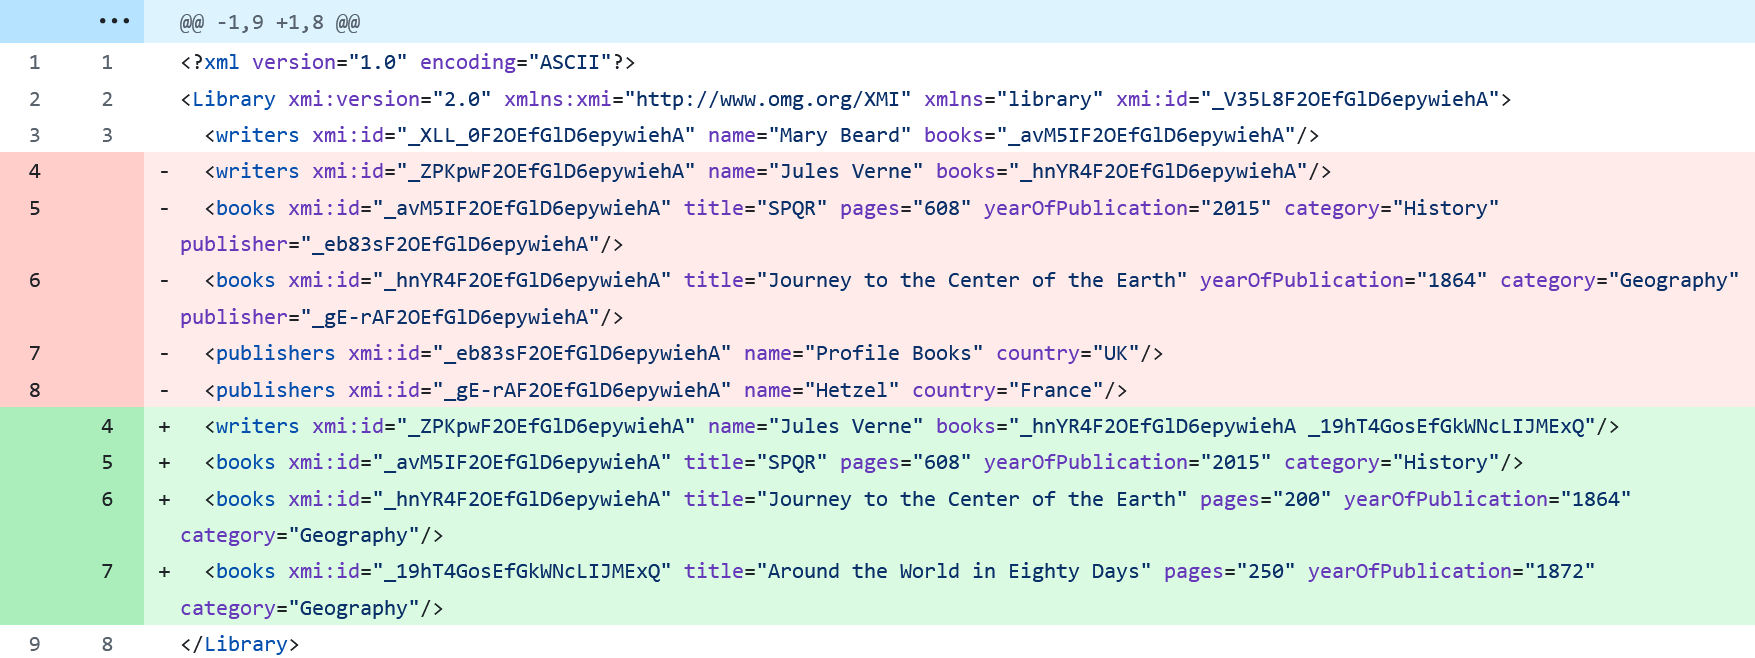
\includegraphics[width=\textwidth]{resources/cambios_textuales_xmi.png}
    \caption{Ejemplo de visualización textual de cambios sobre un modelo serializado en XMI.}
    \label{fig:cambios-textuales-xmi}
\end{figure}

RAMA responde a esta necesidad analizando los archivos como modelos EMF, no únicamente como texto. De este modo, la revisión se aproxima más al significado real de los cambios.

\subsection{Objetivos}

El objetivo principal de este trabajo es facilitar la revisión de cambios en proyectos basados en \textit{Model-Driven Software Engineering}, incorporando información específica sobre modelos y metamodelos al proceso habitual de revisión de código. Para ello, se plantea el desarrollo de RAMA, una herramienta orientada a complementar las diferencias textuales tradicionales con una visión más cercana al significado de los cambios realizados sobre artefactos de modelado.

De este objetivo general se derivan los siguientes objetivos específicos:

\begin{enumerate}
    \item Identificar las limitaciones de los mecanismos habituales de revisión cuando los cambios afectan a modelos o metamodelos representados en formatos textuales.
    \item Diseñar una herramienta capaz de detectar automáticamente los artefactos de modelado modificados y obtener las versiones necesarias para analizarlos en el contexto de un cambio.
    \item Incorporar comparación a nivel de modelo, apoyada en EMF Compare, para obtener información estructural sobre las modificaciones realizadas.
    \item Generar informes a nivel de modelo comprensibles para los revisores, utilizando representaciones de diferencias tanto en formato textual como gráfico.
    \item Integrar RAMA en el flujo de revisión de las \textit{pull requests} en GitHub, de forma que los resultados se publiquen automáticamente como parte de la revisión.
    \item Mantener una arquitectura modular y extensible que facilite la adaptación futura de la herramienta a otros formatos de modelo, proveedores de control de versiones o formatos de informe.
\end{enumerate}

\subsection{Alcance}

El alcance de este trabajo se centra en una primera versión funcional de RAMA integrada en GitHub. La herramienta se ejecuta desde GitHub Actions \cite{github-actions}, obtiene la información de una \textit{pull request}, identifica archivos de modelo y metamodelo según una configuración del repositorio, recupera las versiones del modelo de cada rama comparada, ejecuta comparaciones con EMF Compare y publica un comentario automático con representaciones textuales y gráficas generadas a partir de Munidiff y PlantUML.

La implementación actual contempla modelos y metamodelos EMF serializados en XMI y metamodelos Ecore. También soporta la detección de múltiples archivos de modelos modificados en la misma versión, archivos añadidos y eliminados, archivos renombrados mediante la ruta anterior y la ruta actual, y comparaciones a tres vías cuando existen cambios en dos ramas paralelas que pueden dar lugar a conflictos al intentar fusionarlas. Además, RAMA evita que los errores de un archivo concreto no impidan generar el informe del resto de archivos.

Además de la funcionalidad principal de RAMA, una parte importante del trabajo se ha dedicado a evaluar su correcto funcionamiento en repositorios alojados en GitHub. Para ello, ha sido necesario desarrollar y mejorar herramientas complementarias que permiten preparar escenarios de prueba, generar ramas, \textit{commits} y \textit{pull requests}, y comprobar el comportamiento de RAMA en condiciones cercanas a su uso real. Estas herramientas y su papel dentro del proceso de validación se describen en la Sección~\ref{sec:pruebas} de este trabajo.

El resto de la memoria se organiza de la siguiente forma. La Sección~\ref{sec:antecedentes} presenta los antecedentes necesarios para comprender el contenido técnico del trabajo, incluyendo control de versiones colaborativo, revisiones de código, \textit{Model-Driven Software Engineering} (MDSE), EMF y Munidiff. La Sección~\ref{sec:metodologia-requisitos-arquitectura} describe la metodología seguida, los requisitos planteados y la arquitectura general de RAMA. La Sección~\ref{sec:implementacion} detalla la implementación de la herramienta y el flujo de ejecución completo. La Sección~\ref{sec:pruebas} recoge las pruebas realizadas y los escenarios utilizados para validar el comportamiento de RAMA. Finalmente, la Sección~\ref{sec:conclusiones-trabajo-futuro} resume las conclusiones del trabajo y plantea posibles líneas de mejora.

\newpage

\section{Antecedentes}
\label{sec:antecedentes}

\subsection{Revisión de código y Sistemas de control de versiones colaborativos}

Un sistema de control de versiones permite registrar la evolución de un proyecto a lo largo del tiempo. En Git \cite{progit}, la unidad central de trabajo es el repositorio, que almacena tanto los archivos del proyecto como el historial de cambios realizados sobre ellos. Cada cambio confirmado se introduce mediante un \textit{commit}, que representa una instantánea del estado del proyecto e incluye información sobre su autor, fecha, mensaje descriptivo y relación con los \textit{commits} anteriores.

En proyectos colaborativos, el desarrollo no suele realizarse directamente sobre una única línea de trabajo. Lo habitual es utilizar ramas para aislar cambios relacionados con una funcionalidad, una corrección o una tarea concreta. Una rama parte de un \textit{commit} existente y evoluciona de forma independiente: puede recibir nuevos \textit{commits} mientras la rama principal, normalmente \texttt{main}, continúa avanzando con otros cambios.

Esta separación permite que varios desarrolladores trabajen en paralelo sin bloquearse entre sí. Por ejemplo, una rama puede introducir una nueva funcionalidad mientras otra corrige un error y la rama principal recibe cambios ya validados. Aunque todas procedan de un historial común, cada rama puede modificar archivos distintos o incluso las mismas partes del proyecto. Por ello, el historial deja de ser una única secuencia lineal y pasa a formar una estructura con puntos de divergencia y posterior integración, como se puede observar en la Figura~\ref{fig:ramas-versionado}.

\begin{figure}[htbp]
    \centering
    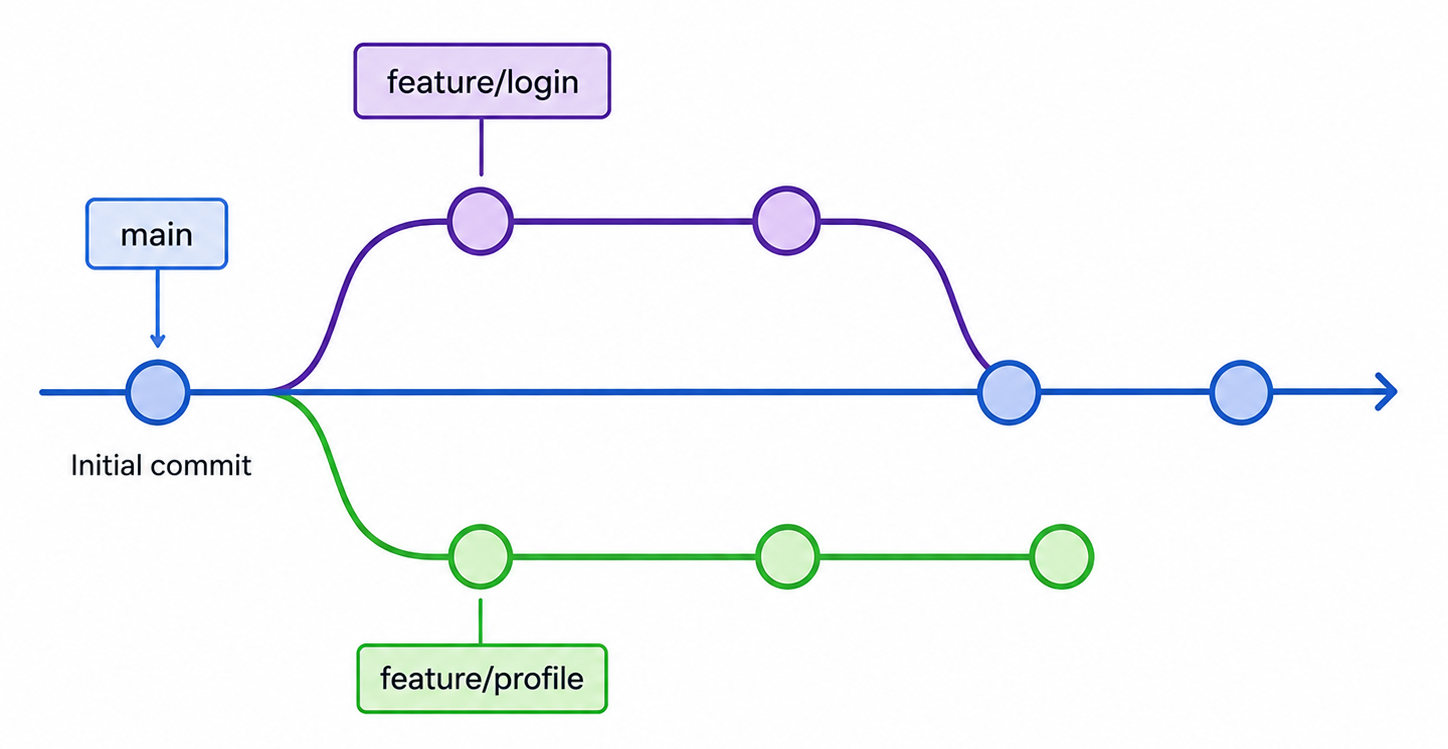
\includegraphics[width=\textwidth]{resources/git_branches.png}
    \caption{Evolución paralela de dos ramas desde un commit común.}
    \label{fig:ramas-versionado}
\end{figure}

Cuando el trabajo de una rama se considera listo para incorporarse a la rama principal, plataformas colaborativas como GitHub utilizan \textit{pull requests} como mecanismo de integración y revisión. Una \textit{pull request} propone fusionar una rama origen en una rama destino, normalmente \texttt{main}, y proporciona un espacio donde inspeccionar los cambios, ejecutar comprobaciones automáticas y discutir posibles ajustes antes de aceptar la integración. Desde el punto de vista técnico, la \textit{pull request} se apoya en la comparación entre ambas ramas; desde el punto de vista del proceso, actúa como una unidad de revisión de código.

En este contexto, es importante entender la terminología relacionada con las ramas y las versiones que se comparan. En una operación de comparación o \textit{merge}, se suelen distinguir tres versiones relevantes:

\begin{verbatim}
source = izquierda / versión nueva
target = derecha / versión antigua
merge-base = versión origin
\end{verbatim}

Una comparación a dos vías utiliza únicamente dos versiones de un archivo o artefacto: una versión antigua y una versión nueva. Este tipo de comparación permite identificar qué ha cambiado entre ambas, y es el caso habitual de un \textit{diff} mostrado en una revisión. Una comparación a tres vías incorpora además una tercera versión común, el \textit{merge-base}, que representa el estado desde el que divergieron las ramas comparadas. Esta información permite distinguir si un cambio procede de la rama origen, de la rama destino o de ambas.

La comparación a tres vías es especialmente importante en operaciones de integración, porque no solo permite calcular diferencias, sino también detectar conflictos. Un conflicto aparece cuando los cambios introducidos en dos ramas no pueden combinarse de forma automática y segura a partir de la versión común. Por tanto, mientras que una comparación a dos vías responde principalmente a la pregunta de qué ha cambiado entre dos versiones, una comparación a tres vías permite razonar sobre cómo se han producido esos cambios en paralelo y si pueden integrarse sin intervención manual.

Los repositorios actuales no solo almacenan historial y facilitan la revisión, sino que también permiten asociar automatizaciones a eventos del proyecto. Es habitual que una \textit{pull request} active procesos de integración continua, como compilación, ejecución de pruebas, análisis estático o validación de configuración, antes de que los cambios se incorporen a la rama principal. Herramientas como GitHub Actions permiten definir estos procesos como \textit{workflows} versionados junto al propio repositorio \cite{github-actions}. En este contexto, RAMA puede entenderse como una automatización asociada al flujo de revisión y, en sentido amplio, como parte del entorno de integración continua del proyecto: se ejecuta automáticamente cuando cambia una \textit{pull request} y publica información útil para decidir si el cambio debe aceptarse.

La integración final puede realizarse mediante una operación de \textit{merge}. Para determinar cómo combinar los cambios, Git compara tres estados: la versión común desde la que ambas ramas divergieron, conocida como \textit{merge-base}; la versión actual de la rama destino o \textit{target}; y la versión actual de la rama origen o \textit{source}. Si las modificaciones realizadas en cada rama afectan a zonas independientes, el sistema suele poder construir automáticamente una versión resultante.

No obstante, pueden aparecer conflictos cuando Git no puede determinar de forma segura cómo combinar ambas ramas. El caso más habitual se produce cuando dos ramas modifican de manera incompatible la misma parte de un archivo desde el mismo origen común. Por ejemplo, si las dos ramas a combinar cambian la misma línea del mismo archivo, pero de manera diferente, el sistema no puede decidir cuál debe prevalecer sin intervención humana. También pueden producirse conflictos cuando una rama elimina una línea que otra ha modificado o cuando se renombran elementos de forma incompatible.

En archivos de texto, las plataformas de revisión muestran las diferencias mediante \textit{diffs} basados en líneas, y los conflictos suelen aparecer con marcas que delimitan la versión de cada rama. RAMA se sitúa precisamente en este punto del flujo: mejora la forma en que se muestran las diferencias de artefactos de modelado en una \textit{pull request}, complementando los mecanismos habituales de comparación textual con información a nivel de modelo.

\subsection{\textit{Model-Driven Software Engineering (MDSE)}}

La Ingeniería del software Dirigida por Modelos o \textit{Model-Driven Software Engineering (MDSE)} es un enfoque de desarrollo de software que sitúa los modelos como elemento central del proceso de ingeniería. La idea fundamental es representar sistemas complejos mediante abstracciones de alto nivel que permitan describir su estructura, comportamiento y restricciones de forma más comprensible \cite{brambilla-mdse}.

En lugar de utilizar modelos solo como documentación, MDSE los trata como artefactos manipulables por herramientas. Estos modelos pueden utilizarse para análisis, validación, transformación, simulación o generación de código. Este paradigma ha ganado relevancia porque los sistemas software modernos son cada vez más complejos, distribuidos y difíciles de mantener, por lo que trabajar con modelos facilita la gestión de dicha complejidad y mejora la comunicación entre desarrolladores, analistas y expertos del dominio.

MDSE se utiliza ampliamente en ámbitos donde la precisión, la reutilización y la automatización son especialmente importantes. Es común en sectores como la automoción \cite{autosar}, la aeronáutica \cite{ieee-aerospace-mdse}, los sistemas embebidos \cite{mbeddr} y el desarrollo de software empresarial \cite{outsystems}. Por ejemplo, en la industria automotriz se emplea para diseñar sistemas de control electrónico, mientras que en entornos empresariales puede utilizarse para generar automáticamente partes de aplicaciones a partir de modelos conceptuales. Su adopción en estos contextos se debe a que permite reducir errores humanos, acelerar el desarrollo y garantizar una mayor coherencia entre diseño e implementación.

Entre sus principales ventajas destaca la capacidad de automatizar transformaciones y generación de código, lo que incrementa la productividad y reduce tareas repetitivas. Además, al trabajar con modelos más cercanos al dominio del problema, se mejora la comprensión del sistema y la comunicación entre perfiles técnicos y no técnicos. También favorece la reutilización de componentes conceptuales y facilita el mantenimiento, ya que modificar un modelo de alto nivel puede resultar más sencillo que intervenir directamente sobre grandes bases de código. Otra ventaja importante es la posibilidad de validar diseños en etapas tempranas del desarrollo, reduciendo costes asociados a errores detectados demasiado tarde.

Sin embargo, MDSE también presenta desafíos y limitaciones. La curva de aprendizaje puede ser elevada, especialmente cuando implica herramientas especializadas, metamodelado o lenguajes específicos de dominio. Además, la dependencia de herramientas concretas puede generar problemas de compatibilidad o dificultad para integrar el enfoque con procesos de desarrollo tradicionales. En algunos proyectos pequeños, el coste inicial de modelar y configurar transformaciones puede superar los beneficios obtenidos. Asimismo, si los modelos no se mantienen sincronizados con la implementación real, pueden perder utilidad rápidamente y convertirse en documentación obsoleta.

En base a lo anterior, \textit{Model-Driven Software Engineering} representa una estrategia poderosa para abordar la complejidad del desarrollo de software moderno mediante abstracción y automatización. Aunque no es una solución universal y su adopción debe evaluarse según el contexto del proyecto, resulta especialmente valiosa en sistemas grandes, críticos o con fuerte necesidad de consistencia y reutilización.

En el contexto de este trabajo, lo relevante de MDSE es que los modelos se persisten y versionan en el mismo repositorio que el código fuente, y por tanto evolucionan junto con el resto del sistema. Por tanto, sus cambios deben revisarse con el mismo nivel de atención que los cambios en código fuente. Sin embargo, al estar serializados en formatos textuales con alta verbosidad y redundancia, generados automáticamente y sin que su lectura por parte de los usuarios finales sea una prioridad, su revisión mediante herramientas convencionales puede resultar insuficiente.

\subsection{Modelos y metamodelos}

Un modelo es una representación abstracta de un sistema, dominio o problema. Puede describir entidades, relaciones, atributos, reglas o comportamiento. En proyectos software, un modelo puede representar desde una estructura de datos hasta un lenguaje específico de dominio.

Un metamodelo define la estructura que deben seguir los modelos. Es decir, describe qué tipos de elementos pueden existir, qué atributos tienen y cómo pueden relacionarse entre sí. Si un modelo es una instancia, el metamodelo actúa como su esquema o lenguaje. La estructura principal de los elementos de un metamodelo es muy similar a la de los diagramas de clases de UML, ya que incluye conceptos como clases, atributos y relaciones. Por ello, es habitual utilizar diagramas de clases para visualizar metamodelos de forma más comprensible.

\subsubsection{\textit{Running example}: Biblioteca}
\label{sec:running-example-biblioteca}

Como ejemplo recurrente de este trabajo se utilizará un dominio sencillo de biblioteca. La Figura~\ref{fig:metamodelo-biblioteca} muestra el metamodelo de este dominio, que define los conceptos principales que pueden aparecer en los modelos: bibliotecas, libros, autores, socios y editoriales. La biblioteca actúa como elemento raíz y contiene colecciones de estos elementos; los libros se relacionan con sus autores y con una editorial, y los socios representan usuarios que pueden formar parte del sistema. Este metamodelo describe, por tanto, el lenguaje con el que se pueden construir modelos concretos de bibliotecas.

\begin{figure}[htbp]
    \centering
    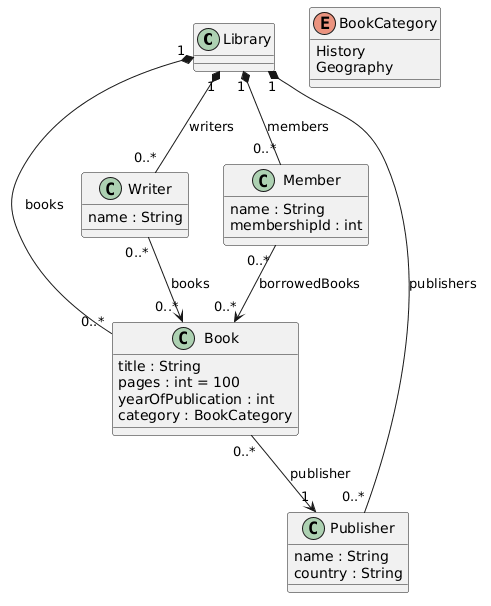
\includegraphics[width=0.60\textwidth]{resources/metamodelo_biblioteca.png}
    \caption{Metamodelo Ecore utilizado como ejemplo de biblioteca.}
    \label{fig:metamodelo-biblioteca}
\end{figure}

La Figura~\ref{fig:modelo-biblioteca} muestra un modelo conforme al metamodelo anterior. En este caso, el modelo representa una biblioteca concreta con dos libros, dos autores, un socio y dos editoriales. Cada elemento del modelo es una instancia de alguno de los tipos definidos en el metamodelo: por ejemplo, los objetos \texttt{book1} y \texttt{book2} son instancias de \texttt{Book}, mientras que \texttt{author1} y \texttt{author2} son instancias de \texttt{Author}. De forma análoga a los metamodelos, que pueden visualizarse mediante diagramas de clases, un modelo concreto puede representarse de forma bastante natural mediante un diagrama de objetos de UML, donde se muestran las instancias y los enlaces entre ellas. Esta relación entre modelo y metamodelo será la base del \textit{running example} empleado más adelante para explicar cómo RAMA analiza cambios en artefactos de modelado.

\begin{figure}[htbp]
    \centering
    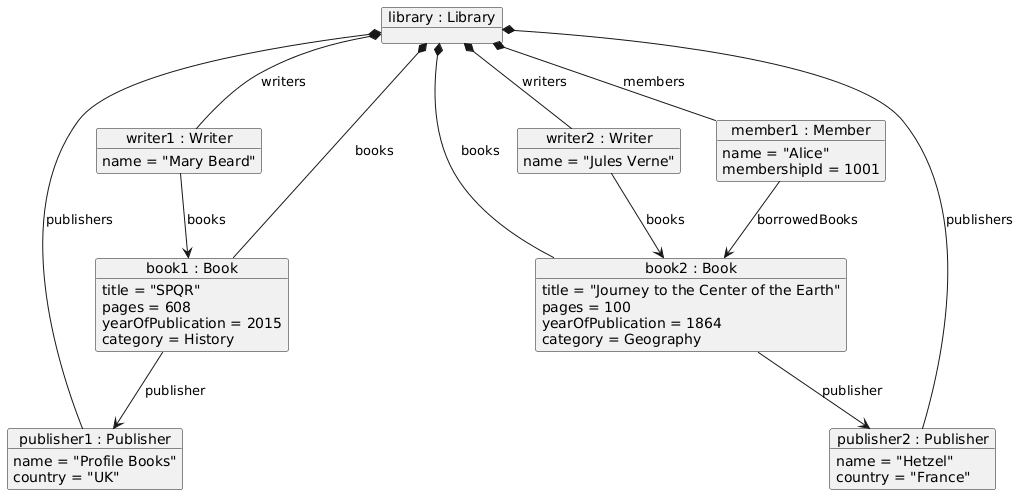
\includegraphics[width=\textwidth]{resources/modelo_biblioteca.png}
    \caption{Modelo de biblioteca conforme al metamodelo del ejemplo.}
    \label{fig:modelo-biblioteca}
\end{figure}

\subsection{\textit{Eclipse Modeling Framework} y XMI}

\textit{Eclipse Modeling Framework (EMF)} es uno de los pilares técnicos más utilizados dentro del ecosistema de desarrollo dirigido por modelos en Eclipse \cite{emf-book,emf-docs}. Proporciona una infraestructura para definir metamodelos, generar código Java a partir de ellos, crear editores básicos y manipular modelos en tiempo de ejecución. Su idea central es que la estructura de los datos de una aplicación puede describirse mediante un modelo y que, a partir de esa descripción, se pueden obtener clases, mecanismos de serialización, reflexión, notificación de cambios y persistencia.

En EMF, los modelos se manipulan como grafos de objetos que conforman a un metamodelo. Estos modelos suelen almacenarse en formatos como XMI (\textit{XML Metadata Interchange}), un formato basado en XML que serializa los objetos del modelo, sus atributos y sus referencias de acuerdo con el metamodelo al que conforman. Esta serialización permite almacenar modelos y metamodelos como archivos textuales, por ejemplo \texttt{.model} o \texttt{.ecore}, y facilita su intercambio entre herramientas EMF y su versionado en repositorios Git. No obstante, el contenido XMI refleja la estructura interna del modelo y no siempre resulta cómodo de interpretar manualmente: las referencias, identificadores y elementos anidados pueden producir diferencias textuales extensas aunque el cambio conceptual sea pequeño.

XMI fue diseñado principalmente como un formato de persistencia e intercambio de modelos entre herramientas de modelado \cite{XMI}. Por ello, su representación está orientada a que las herramientas puedan guardar, cargar y reconstruir modelos de forma sistemática, no a que los usuarios finales trabajen directamente sobre el texto generado. Aspectos como la posibilidad de procesar el documento con analizadores XML estándar, conservar referencias entre elementos o mantener una representación completa del grafo del modelo tienen más peso que la legibilidad humana del archivo.

Esta orientación explica que un fichero XMI pueda contener identificadores generados, referencias internas largas y estructuras repetitivas que son manejables para una herramienta, pero difíciles de revisar manualmente. Incluso cuando el formato resulta adecuado para persistencia, intercambio o versionado como archivo, no proporciona por sí mismo una vista cómoda del significado del modelo. En consecuencia, revisar una modificación únicamente a partir del XMI obliga al revisor a localizar pequeños cambios relevantes dentro de fragmentos textuales extensos y poco expresivos.

Ecore es el lenguaje de metamodelado de EMF. Permite definir paquetes, clases, atributos, referencias, operaciones y otros elementos estructurales que describen la forma que deben tener los modelos. Una característica importante es que Ecore es, al mismo tiempo, un metamodelo y un modelo dentro de EMF: los metamodelos definidos en archivos \texttt{.ecore} son modelos conformes al propio metamodelo Ecore. Por tanto, un archivo \texttt{.ecore} puede tratarse como artefacto de modelado, pero representa la definición de un lenguaje o dominio sobre el que después se construirán otros modelos.

Dentro de RAMA, los archivos \texttt{.ecore} se consideran metamodelos. Cuando una \textit{pull request} modifica uno de estos archivos, la herramienta utiliza un tratamiento específico para metamodelos tanto en la fase de identificación de elementos como en la generación del informe gráfico. Esto permite que los cambios en metamodelos se representen de forma más adecuada que si fueran tratados como modelos genéricos.

\subsection{EMF Compare}

EMF Compare es la herramienta utilizada por RAMA para calcular diferencias entre versiones de modelos EMF \cite{emfcompare-overview,emfcompare-api}. En lugar de comparar líneas de texto, EMF Compare trabaja sobre modelos EMF ya cargados, por lo que puede detectar cambios en elementos, atributos y referencias del modelo.

RAMA crea una comparación con tres entradas:

\begin{itemize}
    \item La versión de la rama fuente de la \textit{pull request}, tratada como versión nueva.
    \item La versión de la rama objetivo, tratada como versión antigua.
    \item La versión del \textit{merge-base}, utilizada como origen común.
\end{itemize}

Esta orientación es importante porque la capa de informes espera que la rama fuente aparezca como la versión nueva y la rama objetivo como la versión antigua. Así, las adiciones y eliminaciones se muestran en la dirección esperada para el revisor.

EMF Compare resuelve, por tanto, la parte de análisis: identifica qué elementos, atributos o referencias han cambiado entre las versiones comparadas. Sin embargo, su representación de resultados está pensada principalmente para utilizarse como parte de un plugin dentro del entorno Eclipse. Esta forma de visualización resulta útil dentro de un entorno de modelado, pero no encaja directamente con una revisión de cambios en una \textit{pull request}, donde el revisor trabaja en GitHub y espera ver la información integrada en la conversación de la revisión. Por ello, además de calcular las diferencias, es necesario transformarlas en informes publicables fuera de Eclipse. En este punto entra Munidiff, que proporciona representaciones textuales y gráficas más adecuadas para integrarse en el flujo de revisión de GitHub.

\subsection{Munidiff}

Munidiff es la capa de representación de diferencias, utilizada para transformar los resultados de EMF Compare en informes más comprensibles \cite{munidiff-paper,munidiff}. En RAMA se reutilizan los informes ofrecidos por Munidiff; en concreto, los informes gráficos de modelos y metamodelos, y los informes textuales de modelos.

El ejemplo de biblioteca presentado en la Sección~\ref{sec:running-example-biblioteca} permite ilustrar estos tipos de informe. En este caso, el modelo \texttt{library-1.model}, que conforma al metamodelo de la Figura~\ref{fig:metamodelo-biblioteca}, contiene cambios sobre las referencias a editoriales y sobre atributos de los libros. A partir de esas diferencias, Munidiff puede generar tanto una vista textual como una vista gráfica. La Figura~\ref{fig:munidiff-modelo-textual} muestra el informe textual, con un formato similar a \texttt{unified diff}: las líneas eliminadas aparecen marcadas en rojo y las líneas añadidas en verde.

\begin{figure}[htbp]
    \centering
    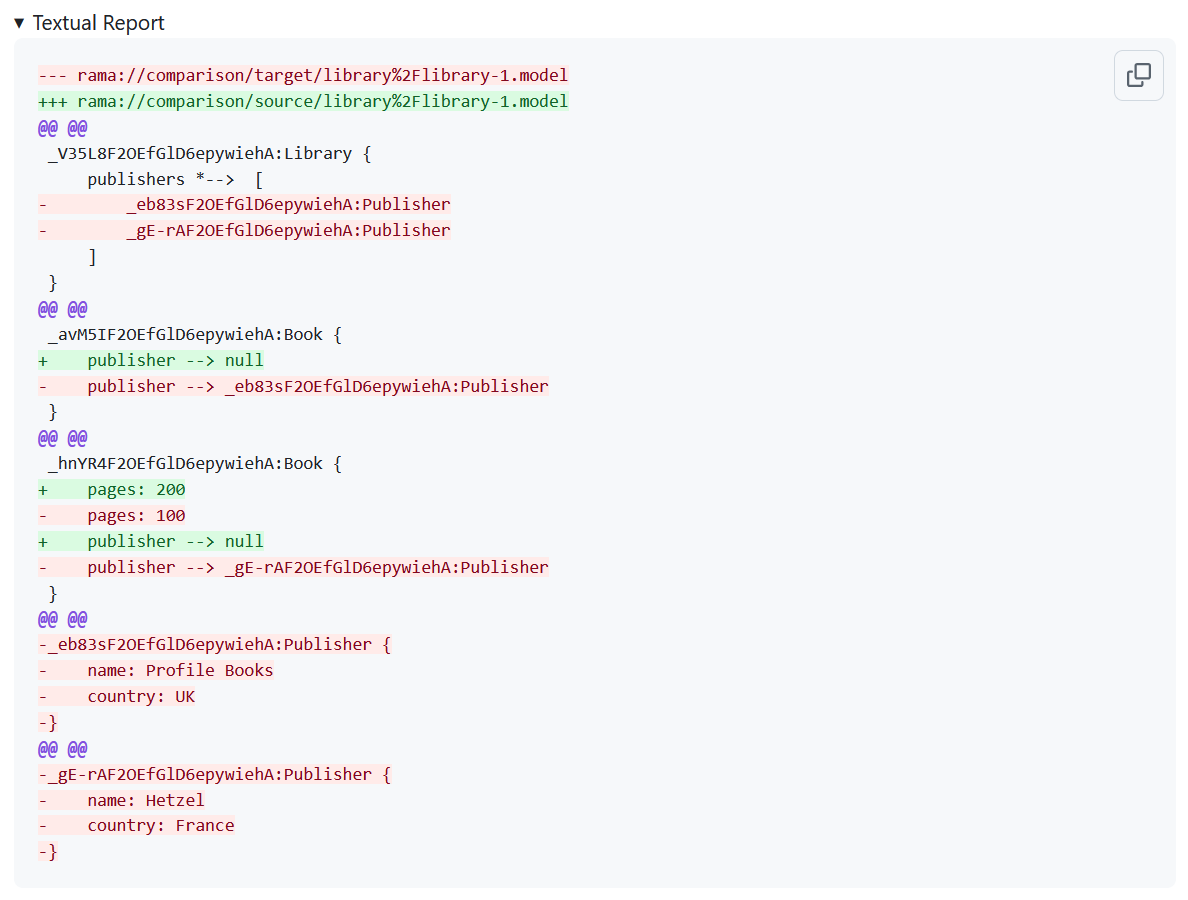
\includegraphics[width=0.9\textwidth]{resources/ejemplo_modelo_textual.png}
    \caption{Ejemplo de informe textual de Munidiff para el modelo \texttt{library-1.model}.}
    \label{fig:munidiff-modelo-textual}
\end{figure}

La misma comparación sobre \texttt{library-1.model} puede representarse también como un informe gráfico de modelo. En esta vista, mostrada en la Figura~\ref{fig:munidiff-modelo-grafico}, los elementos y referencias afectados se presentan como nodos y relaciones del modelo, lo que facilita identificar qué objetos del dominio de biblioteca cambian y cómo se conectan entre sí.

\begin{figure}[htbp]
    \centering
    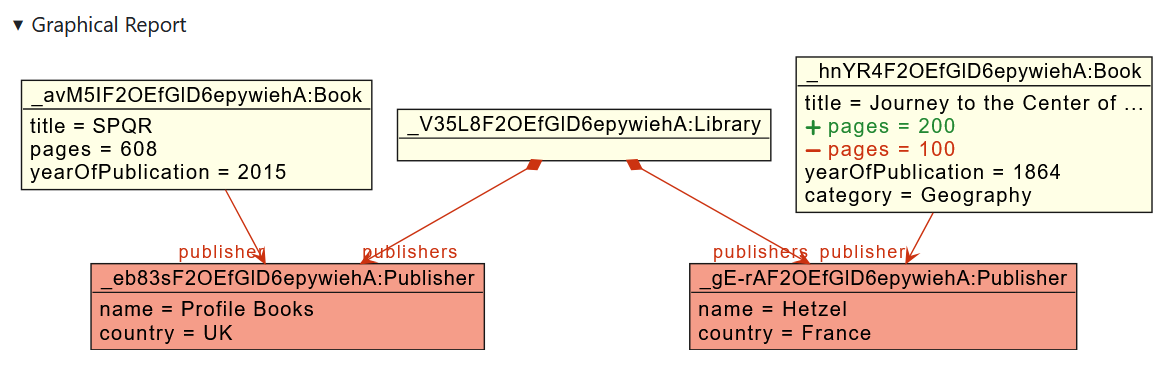
\includegraphics[width=\textwidth]{resources/ejemplo_modelo_grafico.png}
    \caption{Ejemplo de informe gráfico de Munidiff para el modelo \texttt{library-1.model}.}
    \label{fig:munidiff-modelo-grafico}
\end{figure}


Ambas representaciones se generan a partir del mismo resultado de comparación mostrado en la Figura~\ref{fig:munidiff-rendering-example}. Para ello, RAMA toma el resultado producido por EMF Compare y lo transforma en un modelo Munidiff mediante la clase \texttt{EmfCompare2Munidiff}. Este modelo intermedio preserva las diferencias relevantes de forma independiente de su representación final, permitiendo generar posteriormente tanto un informe textual con formato \texttt{unified diff} como una representación gráfica en PlantUML \cite{plantuml}. En este último caso, la descripción PlantUML se renderiza como una imagen SVG mediante un servidor PlantUML, que es la que finalmente se inserta en el comentario de GitHub.

\begin{figure}[htbp]
    \centering
    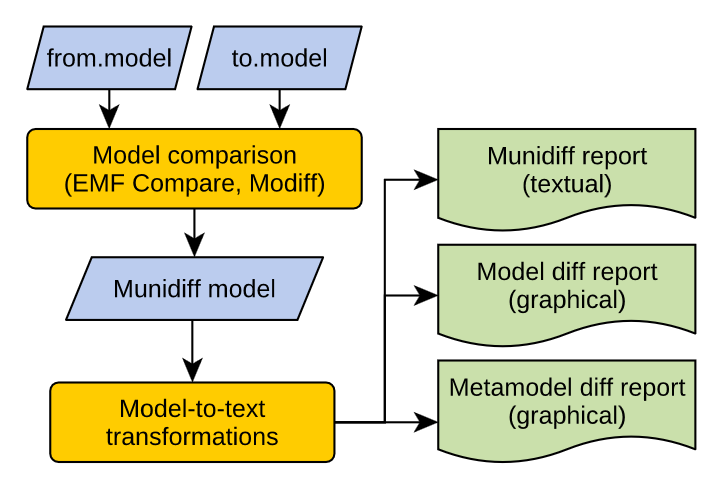
\includegraphics[width=0.75\textwidth]{resources/munidiff_workflow.png}
    \caption{Flujo de generación de informes de diferencias en Munidiff, tomado de \cite{timeline-paper}.}
    \label{fig:munidiff-rendering-example}
\end{figure}

\newpage

\section{Metodología, Requisitos y Arquitectura}
\label{sec:metodologia-requisitos-arquitectura}

\subsection{Metodología de desarrollo}

El desarrollo de RAMA se planteó de forma incremental, partiendo de un primer prototipo que diera soporte flujo completo de la herramienta antes de ampliarlo a todos los casos particulares. Por ello, en lugar de implementar por completo todos los componentes de forma aislada, se priorizó una versión mínima capaz de ejecutarse en una \textit{pull request}, seleccionar un archivo de modelo modificado, obtener sus versiones, compararlas con EMF Compare y publicar un comentario en GitHub.

Este enfoque permitió validar pronto las decisiones principales de integración: el arranque desde GitHub Actions, el acceso a la API de GitHub, la carga de configuración de RAMA, la recuperación de contenidos de ramas distintas, la comparación de modelos EMF y la publicación del informe. Una vez comprobado ese flujo completo, la implementación se fue incrementalmente ampliando para cubrir varios archivos, metamodelos Ecore, versiones de \textit{merge-base} para realizar comparaciones a tres vías, conflictos detectados por EMF Compare, renombrados, archivos ausentes y manejo de errores por archivo.

La metodología seguida puede resumirse en tres ideas. Primero, construir una versión ejecutable de extremo a extremo, aunque inicialmente tuviera un alcance reducido. Segundo, mantener fronteras claras entre integración con GitHub, comparación de modelos y generación de informes, para poder evolucionar cada parte sin afectar el resto. Tercero, convertir los fallos detectados durante las pruebas en mejoras del flujo de ejecución, especialmente en el tratamiento de errores y en la generación de diagnósticos para el revisor.

\subsection{Requisitos funcionales y no funcionales}

RAMA se ha diseñado como una aplicación Java ejecutable desde un \textit{workflow} de GitHub Actions \cite{github-actions}. El flujo comienza cuando se abre, actualiza o reabre una \textit{pull request} en un repositorio de GitHub. El \textit{workflow} compila la herramienta y la ejecuta pasando como argumento el identificador de la \textit{pull request} a procesar.

Desde el punto de vista de requisitos funcionales, en cada ejecución RAMA lleva a cabo las siguientes operaciones:

\begin{enumerate}
    \item Ejecutarse automáticamente en las \textit{pull requests}.
    \item Identificar archivos relevantes según una configuración del repositorio y obtener las versiones necesarias para realizar una comparación de dos o tres vías.
    \item Comparar los modelos a nivel de contenido, no solo textual.
    \item Generar informes visuales comprensibles y publicarlos como comentarios cronológicos en la \textit{pull request}.
\end{enumerate}

Además de lo anterior, RAMA debe cumplir varios requisitos no funcionales relacionados con su integración en el flujo de trabajo, su accesibilidad y su utilidad durante la revisión:

\begin{enumerate}
    \item La herramienta debe poder ejecutarse sin desplegar ni mantener infraestructura externa adicional.
    \item Los comentarios generados deben estar escritos en inglés, de forma que puedan ser comprendidos en proyectos con equipos internacionales y resulten reutilizables en repositorios con colaboradores de distintos contextos.
    \item La información añadida a la \textit{pull request} debe ser clara, concisa y poco intrusiva. El informe debe presentar primero una visión general del resultado y permitir acceder progresivamente a detalles adicionales, evitando dificultar la tarea principal del revisor.
\end{enumerate}

Este primer requisito condicionó especialmente la decisión de integración con GitHub. Una posibilidad era implementar RAMA como una GitHub App, lo que también habría permitido reaccionar a eventos del repositorio y publicar comentarios en las \textit{pull requests}. Sin embargo, esta opción exige disponer de un servicio externo que reciba los eventos, gestione la autenticación de la aplicación y ejecute la lógica de análisis. Frente a ello, GitHub Actions permite ejecutar RAMA directamente dentro del entorno proporcionado por el repositorio, reutilizando el sistema de permisos, secretos y eventos de GitHub. Por esta razón se optó por GitHub Actions: reduce la infraestructura que debe mantenerse, y facilita que cualquier proyecto pueda activar la herramienta simplemente mediante la copia del \textit{workflow} generado como parte de las contribuciones de este proyecto

\subsection{Arquitectura}

La arquitectura de RAMA se organiza en tres grandes bloques.

\begin{enumerate}
    \item El primero es el bloque de descubrimiento y selección de archivos de la \textit{pull request}. Este bloque lee la configuración del repositorio, consulta GitHub, obtiene los archivos modificados y decide cuáles son relevantes para el análisis.
    \item El segundo es el bloque de análisis por archivo. Su responsabilidad es reunir las versiones necesarias de cada artefacto, cargarlas como recursos EMF, registrar los metamodelos configurados y ejecutar EMF Compare para obtener diferencias y conflictos a nivel de modelo.
    \item El tercero es el bloque de generación y publicación del informe. Este transforma los resultados de comparación en salidas comprensibles para el revisor y publica un nuevo comentario en la \textit{pull request}.
\end{enumerate}

La Figura~\ref{fig:rama-arquitectura-general} resume esta división y muestra las principales clases e interfaces que materializan cada bloque.

Dentro de esta arquitectura, \texttt{Main} actúa como punto de entrada y crea las dependencias principales, mientras que \texttt{RamaApplication} coordina el flujo de ejecución. \texttt{ConfigService} gestiona la configuración a través de un objeto \texttt{RamaConfig} que se pasa al coordinador \texttt{RamaApplication}. La interfaz \texttt{GitService}, implementada por \texttt{GitHubService}, concentra el descubrimiento y la selección de archivos relevantes de la \textit{pull request}, así como la publicación del comentario final. La interfaz \texttt{ComparisonService}, implementada por \texttt{EmfModelComparator}, encapsula el análisis de cada archivo mediante EMF Compare. Finalmente, \texttt{MunidiffRenderer}, \texttt{PlantUMLEncoderService} y \texttt{ReportCommentRenderer} transforman el resultado de la comparación en una representación publicable en GitHub.

\begin{figure}[htbp]
    \centering
    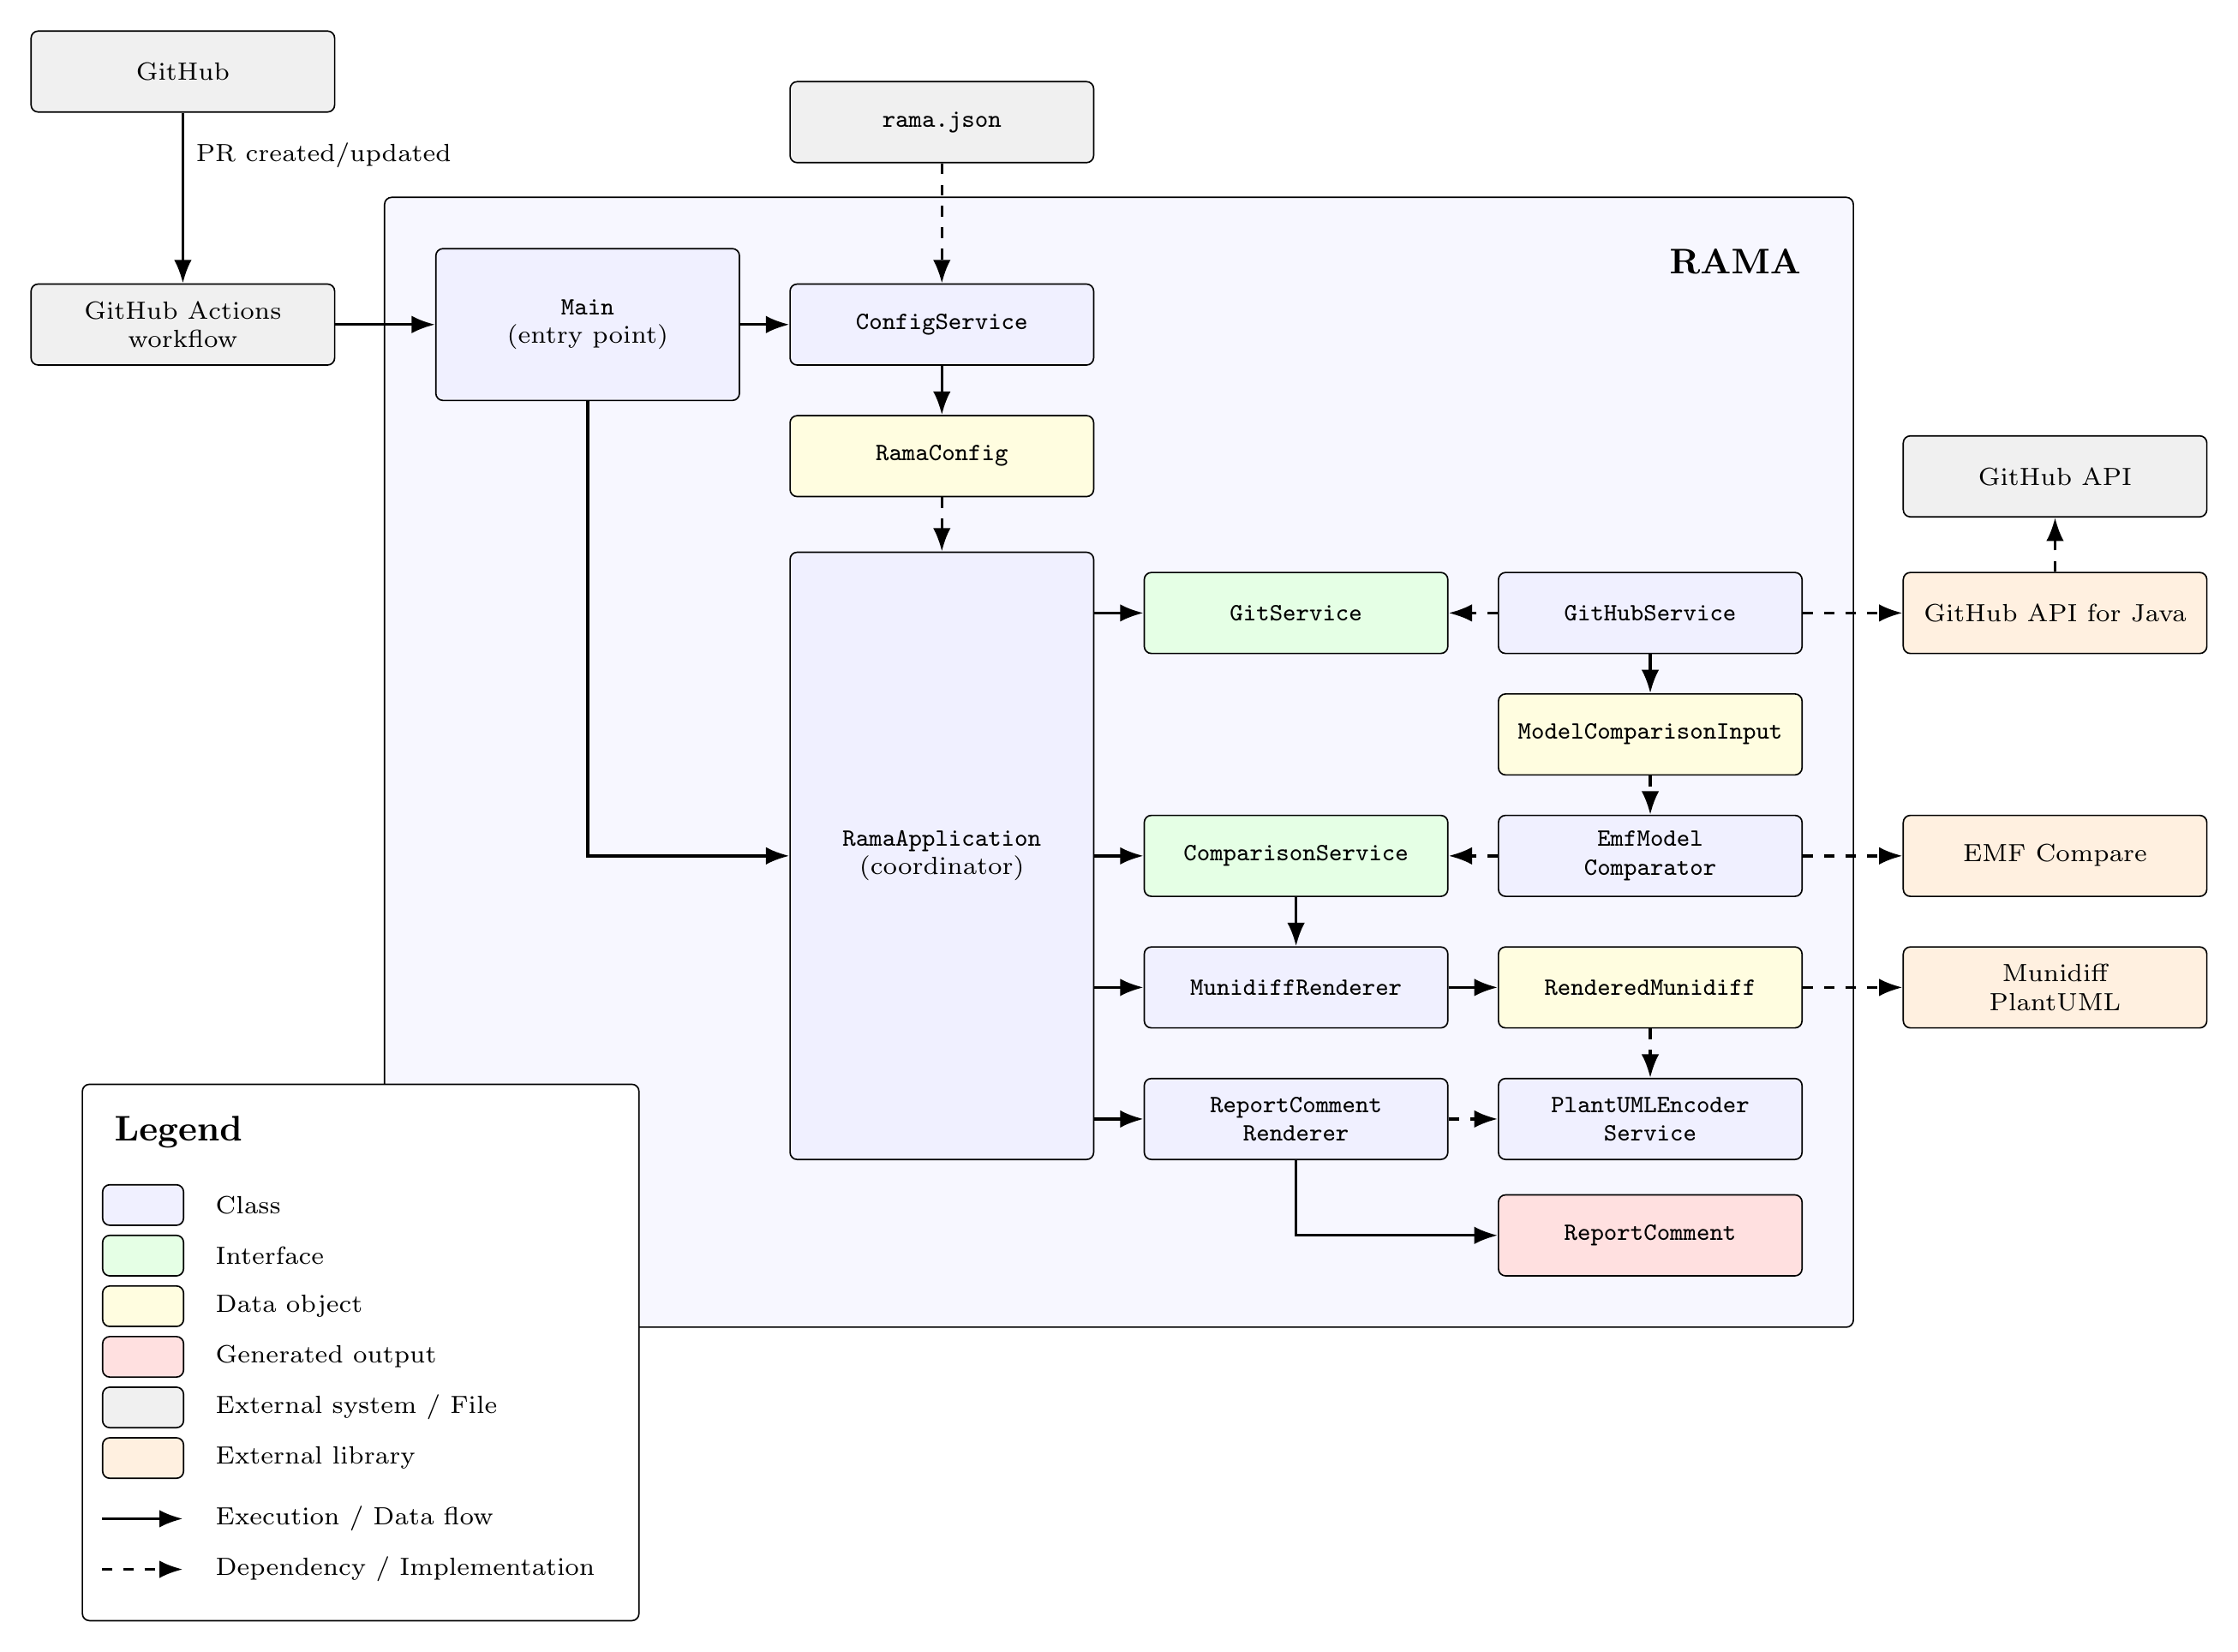
\includegraphics[width=\textwidth]{resources/rama_architecture_general}
    \caption{Arquitectura general de RAMA y principales interfaces de integración.}
    \label{fig:rama-arquitectura-general}
\end{figure}

Esta separación permite que la herramienta sea extensible. Por ejemplo, otro proveedor de control de versiones podría integrarse implementando \texttt{GitService}, y otro mecanismo de comparación podría incorporarse implementando \texttt{ComparisonService}.

\subsection{Flujo de trabajo}

La Figura~\ref{fig:rama-startup} muestra el flujo de alto nivel que sigue RAMA desde que se produce un cambio en una \textit{pull request} hasta que comienza el análisis de los archivos afectados. El proceso se inicia cuando GitHub detecta un evento de \textit{pull request}, como su apertura, reapertura o sincronización tras nuevos \textit{commits}. En el \textit{workflow} de ejemplo se emplea el evento \texttt{pull\_request\_target}; por tanto, el \textit{checkout} sin una referencia explícita deja en el \textit{workspace} la revisión de la rama objetivo. RAMA obtiene posteriormente, mediante la API de GitHub, los contenidos \textit{source}, \textit{target} y \textit{merge-base} que analiza.

\begin{figure}[htbp]
    \centering
    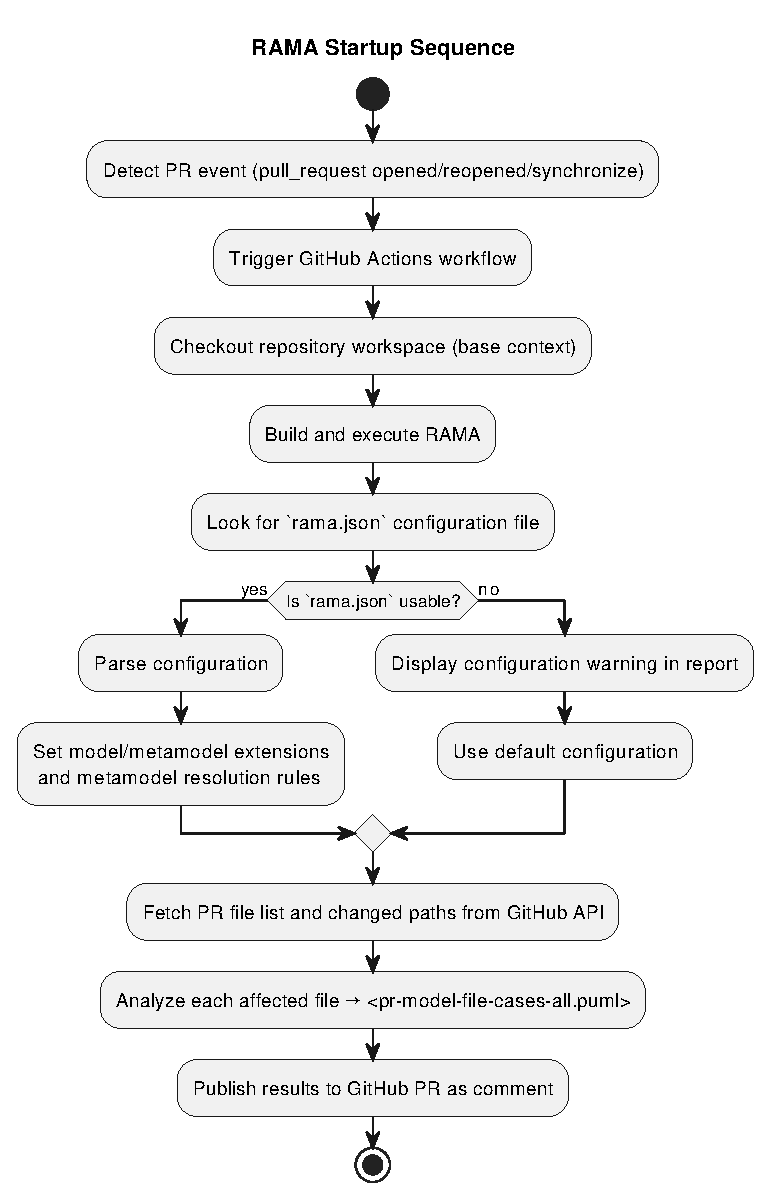
\includegraphics[width=0.66\textwidth]{resources/startup.pdf}
    \caption{Flujo de alto nivel de arranque de RAMA en una \textit{pull request}.}
    \label{fig:rama-startup}
\end{figure}

Una vez iniciada la aplicación, RAMA busca el archivo de configuración \texttt{rama.json}. Si el archivo no existe en el \textit{workspace}, está vacío, no se puede leer o contiene JSON inválido, carga la configuración por defecto empaquetada en el \textit{jar} y añade una advertencia de configuración al comentario de la \textit{pull request}. Si el fichero es válido, Jackson lo deserializa y se utiliza para fijar las extensiones de modelos y metamodelos, así como las rutas de resolución de metamodelos. Con una configuración disponible, RAMA consulta la API de GitHub para recuperar la lista de archivos modificados en la \textit{pull request} y procesa cada archivo relevante por separado, siguiendo el flujo resumido en la Figura~\ref{fig:rama-analisis-archivo}.

\begin{figure}[htbp]
    \centering
    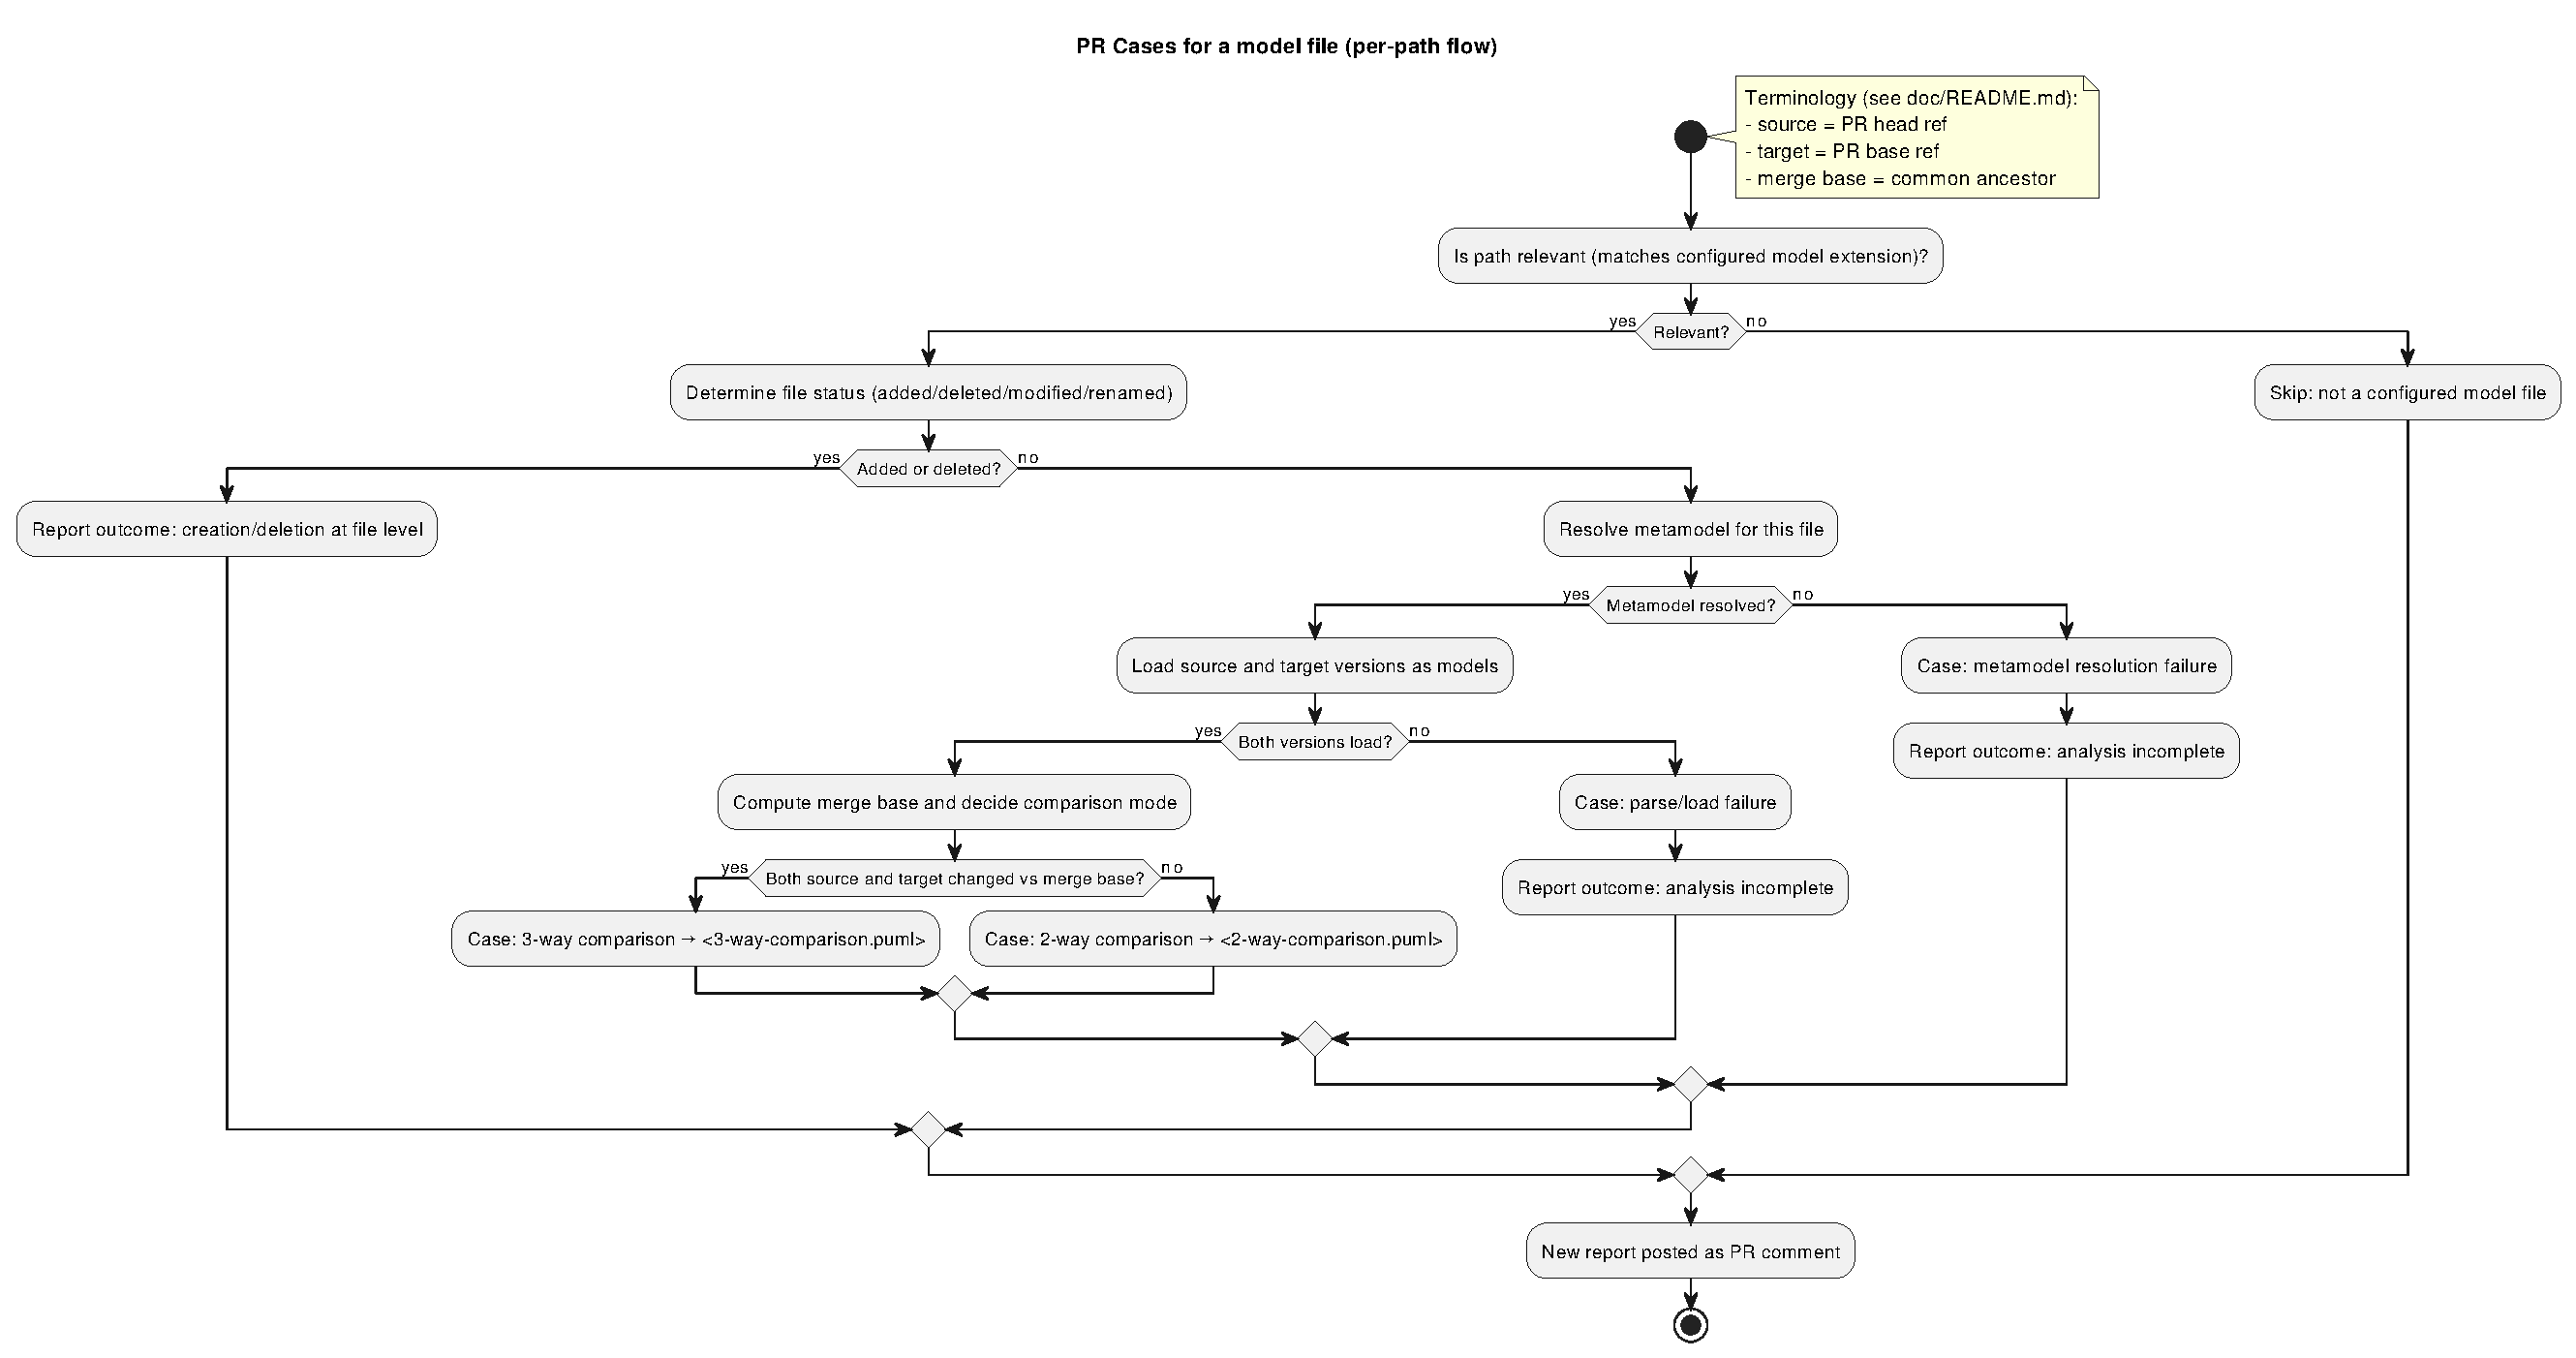
\includegraphics[width=\textwidth]{resources/pr_model_file_cases_all.pdf}
    \caption{Flujo de análisis por archivo de RAMA.}
    \label{fig:rama-analisis-archivo}
\end{figure}

El flujo de la Figura~\ref{fig:rama-analisis-archivo} se aplica de forma independiente a cada ruta modificada en la \textit{pull request}. Primero se comprueba si la ruta coincide con alguna de las extensiones configuradas para modelos o metamodelos. Si no coincide, RAMA descarta el archivo porque no puede aportar información al análisis de modelos. Si coincide, se consulta el estado del archivo en la revisión: los archivos añadidos o eliminados se informan directamente como altas o bajas a nivel de fichero, ya que no hay dos versiones completas que comparar como modelos.

Cuando el archivo sigue existiendo en las versiones necesarias, RAMA intenta resolver el metamodelo que permite cargarlo. Si el metamodelo se encuentra, carga las versiones \textit{source} y \textit{target} como recursos EMF y utiliza la versión \textit{merge-base} para decidir el tipo de comparación. Si tanto la rama fuente como la rama objetivo han cambiado respecto a esa base común, se realiza una comparación de tres vías para poder detectar conflictos. Si solo una de las ramas ha cambiado, o no hay base disponible, se usa una comparación de dos vías. En cualquier punto en el que falle la resolución del metamodelo o la carga del modelo, el archivo no bloquea el resto del análisis: RAMA marca su resultado como incompleto y continúa con los demás archivos. Al final, todos los resultados se agrupan en un nuevo comentario publicado en la \textit{pull request}.

\newpage

\section{Implementación}
\label{sec:implementacion}

El código fuente de RAMA se encuentra disponible en el siguiente repositorio público: \url{https://github.com/sdiaz1208/rama}.

La implementación se explica a partir del repositorio de biblioteca descrito en la Sección~\ref{sec:running-example-biblioteca}. Este repositorio contiene un metamodelo \texttt{library.ecore} y un modelo \texttt{library-1.model} conforme a dicho metamodelo.

La explicación toma como referencia una \textit{pull request} que introduce cambios sobre estos artefactos: por ejemplo, la incorporación de un atributo a la clase \texttt{Book}, la actualización de los datos de un libro existente o la creación de un nuevo préstamo en el modelo. A partir de este escenario, RAMA permite presentar al revisor las diferencias calculadas sobre los elementos EMF reales, evitando que el análisis dependa exclusivamente de la interpretación directa del XMI serializado.

Para seguir el \textit{workflow} descrito en esta sección deben leerse conjuntamente las Figuras~\ref{fig:rama-arquitectura-general} y~\ref{fig:rama-startup}. La primera identifica los componentes, sus interfaces y las dependencias entre ellos; la segunda sitúa esos componentes en la secuencia de ejecución, desde el evento de la \textit{pull request} y el \textit{workflow} de GitHub Actions hasta el inicio del análisis. En particular, el flujo parte de GitHub Actions, entra por \texttt{Main}, construye los servicios de configuración y Git, y los entrega a \texttt{RamaApplication}, que coordina la obtención, comparación y presentación de los resultados.

\subsection{\texttt{Main}: composición de la ejecución}

Como se puede observar en la Figura~\ref{fig:rama-startup}, el punto de partida es el evento de la \textit{pull request}, que causa el arranque de la \textit{GitHub Action} y la compilación de RAMA. A partir de ahí, la ejecución comienza en \texttt{Main}. La Figura~\ref{fig:rama-arquitectura-general} muestra que este punto de entrada no participa en el análisis, sino que compone los servicios que utilizará el coordinador. RAMA se invoca con el número de la \textit{pull request} para tener acceso a la información de la revisión y a los archivos modificados.

\begin{verbatim}
java -jar target/RAMA.jar <pull-request-number>
\end{verbatim}

En el ejemplo de biblioteca de la Sección~\ref{sec:running-example-biblioteca}, este número identifica la \textit{pull request} que contiene los cambios sobre \texttt{library.ecore} y \texttt{library-1.model}. \texttt{Main} no compara modelos ni accede directamente a GitHub. Su responsabilidad es construir las dependencias principales: carga la configuración con \texttt{ConfigService}, crea el servicio Git concreto, instancia \texttt{EmfModelComparator} y prepara los servicios de renderizado. Para ello, la aplicación utiliza las variables de entorno \texttt{GITHUB\_TOKEN}, \texttt{GITHUB\_REPOSITORY} y \texttt{GITHUB\_WORKSPACE}: las dos primeras permiten autenticarse y localizar el repositorio bajo análisis, mientras que la tercera permite resolver la configuración del proyecto en el \textit{workspace} del \textit{workflow}. Finalmente, \texttt{Main} entrega estas dependencias a \texttt{RamaApplication}, que coordina el caso de uso.

Esta separación convierte el arranque en una fase de composición. La lógica de análisis queda concentrada en servicios intercambiables y no en el punto de entrada de la aplicación.

\subsection{Configuración de RAMA}

El primer dato necesario para analizar una \textit{pull request} es saber qué archivos deben tratarse como modelos o metamodelos. Para ello, RAMA busca el archivo \texttt{rama.json} en una ruta concreta del repositorio analizado. Si no existe, está vacío, no se puede leer o contiene JSON inválido, \texttt{ConfigService} carga la configuración por defecto empaquetada en el \textit{jar} y devuelve una advertencia que \texttt{RamaApplication} incorpora al comentario final. Si el fichero es válido, se usa su configuración sin advertencia. En el \textit{workflow} proporcionado, el espacio de trabajo de RAMA corresponde a la rama objetivo; por ello, ni los cambios propuestos en \texttt{rama.json} ni la versión propuesta de un metamodelo cargado mediante \texttt{metamodels} se usan al configurar y cargar otros modelos. El análisis del propio metamodelo modificado, si figura entre los archivos de la revisión, sí usa el contenido recuperado mediante la API. En la Figura~\ref{fig:rama-arquitectura-general}, esta fase se materializa en \texttt{ConfigService} y el objeto \texttt{RamaConfig}, que queda disponible para \texttt{RamaApplication}.

En el fichero \texttt{rama.json} se indican las extensiones de ficheros que RAMA debe considerar que almacenan modelos, las extensiones RAMA que debe considerar que almacenan metamodelos y, opcionalmente, las rutas de los metamodelos que deben registrarse antes de cargar los modelos. Este último punto es importante porque los modelos a cargar pueden ser de un lenguaje de modelado concreto, generalmente definido en un metamodelo personalizado del repositorio. Por ello, deben identificarse explícitamente los metamodelos a cargar para que la carga y procesado de modelos posterior sea satisfactoria.

Para el ejemplo de la Sección~\ref{sec:running-example-biblioteca}, que utiliza modelos \texttt{.model}, metamodelos \texttt{.ecore} y un metamodelo propio \texttt{resources/metamodels/library.ecore}, se podría usar la siguiente configuración:

\begin{lstlisting}[caption={Ejemplo de configuración de RAMA.},label={lst:rama-config}]
{
  "model_extensions": [".model"],
  "metamodel_extensions": [".ecore"],
  "metamodels": ["resources/metamodels/library.ecore"]
}
\end{lstlisting}

El campo \texttt{metamodels} se utiliza más adelante durante la carga EMF. En el ejemplo de la Sección~\ref{sec:running-example-biblioteca}, indica que \texttt{library.ecore} debe registrarse antes de cargar \texttt{library-1.model}, ya que el modelo de la Figura~\ref{fig:modelo-biblioteca} es conforme al metamodelo de la Figura~\ref{fig:metamodelo-biblioteca}.

\subsection{Obtención de versiones desde GitHub}

Una vez cargada la configuración, RAMA consulta GitHub para obtener la lista de archivos modificados en la \textit{pull request}. Esto se corresponde con el paso 10 del flujo representado en la Figura~\ref{fig:rama-startup}. Como muestra la Figura~\ref{fig:rama-arquitectura-general}, \texttt{RamaApplication} accede a esta capacidad a través de \texttt{GitService}, mientras que \texttt{GitHubService} concreta la comunicación con la API de GitHub y produce los \texttt{ModelComparisonInput} que alimentan el análisis.

\texttt{GitService} (Figura~\ref{fig:gitservice-methods}) define la interfaz mínima que RAMA necesita de un proveedor Git: obtener los archivos relevantes de una \textit{pull request} y publicar el comentario final. La implementación actual, \texttt{GitHubService}, usa la librería \texttt{github-api} y se trabaja con los parámetros específicos \texttt{GITHUB\_TOKEN} y \texttt{GITHUB\_REPOSITORY} para la obtención de datos del repositorio y la escritura de mensajes en las \textit{pull requests}.

\begin{figure}[htbp]
    \centering
    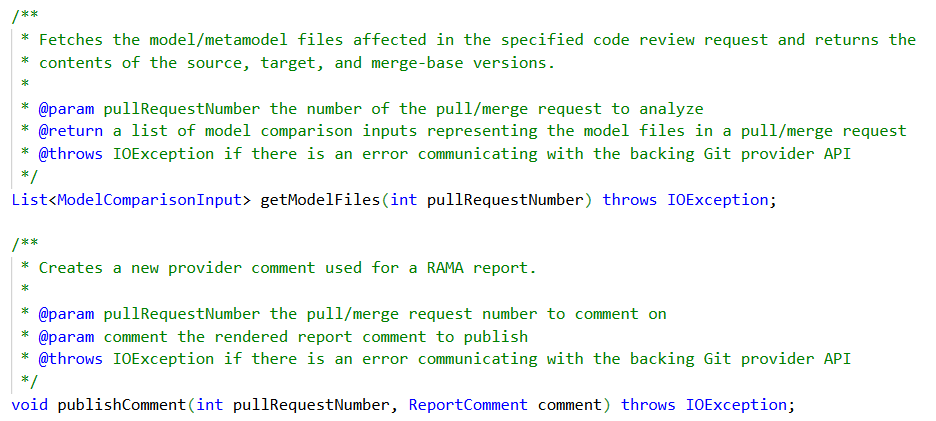
\includegraphics[width=0.9\textwidth]{resources/gitservice_methods.png}
    \caption{Métodos de la interfaz \texttt{GitService}.}
    \label{fig:gitservice-methods}
\end{figure}

En el ejemplo de la Sección~\ref{sec:running-example-biblioteca}, \texttt{GitHubService} obtiene la \textit{pull request} y localiza la rama fuente, que contiene los cambios propuestos, y la rama objetivo, contra la que se quiere integrar. Después calcula el \textit{merge-base commit} entre ambas ramas. Esta tercera versión es necesaria para determinar si la comparación debe ser a dos o a tres vías; si ambas ramas han incluido cambios desde la base común, EMF Compare puede detectar conflictos y RAMA genera un informe con dos vistas laterales, una para cada rama.

A continuación, la clase recorre los archivos modificados. Si la \textit{pull request} contiene por ejemplo \texttt{library-1.model}, \texttt{library.ecore} y \texttt{README.md}, solo los dos primeros superan el filtro de \texttt{RamaConfig}.


Para cada archivo relevante se recuperan tres contenidos: la versión de la rama fuente, la versión de la rama objetivo y la versión del \textit{merge-base}. En un archivo renombrado, RAMA usa la ruta actual para leer la versión fuente y la ruta anterior para leer las versiones objetivo y base. Si GitHub devuelve que el archivo no existe en alguna versión (ver Cuadro~\ref{tab:null-file-versions}), el contenido se representa como \texttt{null}. Este caso aparece, por ejemplo, cuando la \textit{pull request} añade por primera vez un nuevo modelo o elimina uno existente. Cuando falta la versión fuente, el archivo no es un renombrado y existe alguna versión objetivo o base, RAMA lo informa como eliminado y no invoca EMF Compare para ese archivo.

\begin{table}[h]
\centering
\begin{tabular}{|p{0.12\textwidth}|p{0.12\textwidth}|p{0.14\textwidth}|p{0.48\textwidth}|}
\hline
\textbf{source} & \textbf{target} & \textbf{merge-base} & \textbf{Interpretación} \\
\hline
\texttt{no null} & \texttt{null} & \texttt{null} & El fichero no existía en la rama objetivo ni en la base común, por lo que se interpreta como un fichero añadido en la rama fuente. \\
\hline
\texttt{null} & \texttt{no null} & \texttt{no null} & El fichero existía en la rama objetivo y en la base común, pero no en la rama fuente, por lo que se informa como un fichero eliminado en la rama fuente, sin comparación EMF. \\
\hline
\texttt{no null} & \texttt{null} & \texttt{no null} & El fichero existía en la base común, pero ya no existe en la rama objetivo. Este caso indica una eliminación en la rama objetivo, no una adición simple de la rama fuente. \\
\hline
\texttt{null} & \texttt{no null} & \texttt{null} & El fichero no existía en la base común ni en la rama fuente, pero sí en la rama objetivo. Aunque esta combinación refleja una adición en la rama objetivo, la implementación la informa como fichero eliminado porque no hay versión fuente. \\
\hline
\end{tabular}
\caption{Interpretación de combinaciones con versiones ausentes durante la obtención de contenidos desde GitHub.}
\label{tab:null-file-versions}
\end{table}

El resultado de esta fase es una lista de objetos \texttt{ModelComparisonInput} (Figura~\ref{fig:model-comparison-input}). Cada objeto contiene el nombre del archivo y los tres contenidos que necesita la fase de comparación.

\begin{lstlisting}[caption={Estructura de \texttt{ModelComparisonInput}.},label={lst:model-comparison-input}]
public record ModelComparisonInput(
  String filename,
  String previousFilename,
  String sourceContent,
  String targetContent,
  String baseContent
)
\end{lstlisting}

\subsection{Coordinación y tolerancia a fallos}

\texttt{RamaApplication} es el coordinador principal. Su posición central en la Figura~\ref{fig:rama-arquitectura-general} refleja que, una vez completado el arranque de la Figura~\ref{fig:rama-startup}, encadena las fases de obtención, comparación, renderizado y publicación. Para la \textit{pull request} del ejemplo de la Sección~\ref{sec:running-example-biblioteca}, primero solicita a \texttt{GitService} la lista de \texttt{ModelComparisonInput}. Después procesa cada archivo por separado. Para \texttt{library.ecore} y \texttt{library-1.model}, salvo que se clasifiquen como eliminados sin renombre, llama a \texttt{ComparisonService}, entrega el resultado a \texttt{MunidiffRenderer} y acumula un \texttt{FileReport} con la salida que se mostrará al revisor.

La clase también concentra la política de errores. Si falla la obtención inicial de archivos, RAMA no puede continuar con el análisis y publica un comentario de fallo general. Si falla un archivo concreto, por ejemplo porque \texttt{library-1.model} no puede cargarse como XMI válido, el resto de archivos sigue procesándose. El informe final conserva una sección para el archivo fallido con un diagnóstico breve y remite a los logs de GitHub Actions para el detalle completo.

\subsection{Comparación con EMF}

\texttt{ComparisonService} separa la aplicación del mecanismo concreto de comparación. En esta versión de RAMA, la implementación es \texttt{EmfModelComparator}, que compara modelos EMF mediante EMF Compare. La ruta entre \texttt{GitService}, \texttt{ModelComparisonInput}, \texttt{ComparisonService} y EMF Compare se representa en la Figura~\ref{fig:rama-arquitectura-general}. La frontera entre GitHub y EMF es \texttt{ModelComparisonInput}: GitHub entrega cadenas de texto y el comparador se ocupa de cargarlas como recursos EMF.

RAMA realiza la comparación de cada modelo de forma aislada, evitando que el análisis de otros modelos modificados en la misma \textit{pull request} pueda afectar al resultado. Antes de cargar los modelos, el comparador registra los metamodelos configurados. Las rutas relativas, como \texttt{library.ecore}, se resuelven respecto al workspace del repositorio. Cada \texttt{EPackage} cargado se añade al registro de paquetes correspondiente, incluyendo subpaquetes de forma recursiva.

Después se cargan las versiones del archivo. RAMA crea siempre recursos \textit{source} y \textit{target}, incluso cuando sus contenidos son \texttt{null}, en cuyo caso quedan vacíos. El recurso \textit{merge-base} solo se crea si su contenido está disponible; en caso contrario se pasa \texttt{null} a EMF Compare y la comparación es de dos vías. Las eliminaciones sin renombre se detectan antes de esta fase y se informan sin comparar. RAMA asigna una URI sintética a cada recurso cargado para distinguir su lado de la comparación:

\begin{verbatim}
source = izquierda / versión nueva
target = derecha / versión antigua
merge-base = versión origin
\end{verbatim}

Esta orientación es importante para que las capas posteriores interpreten correctamente las altas y modificaciones desde el punto de vista de la \textit{pull request}.

El resultado de la comparación llevada a cabo por EMF Compare contiene las diferencias encontradas entre los modelos y, si existen, los conflictos detectados entre las ramas.

\subsubsection{Comparación con conflictos}

Cuando EMF Compare detecta conflictos en una comparación de tres vías, la aplicación no genera solo un diagrama general. En su lugar, vuelve a comparar los cambios de la rama fuente contra la base y los cambios de la rama objetivo contra la base. Así puede construir un informe de conflicto con dos vistas laterales, una para cada rama.

Por ejemplo, continuando con el \textit{running example} de la Sección~\ref{sec:running-example-biblioteca}, si se cambia el mismo atributo con diferentes valores en ambas ramas de una \textit{pull request}, RAMA lo interpreta como un conflicto y genera un informe como el de la Figura~\ref{fig:cambios-conflicto}.

\begin{figure}[htbp]
    \centering
    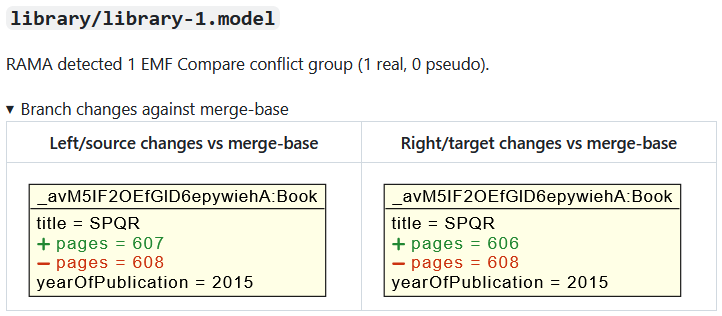
\includegraphics[width=\textwidth]{resources/cambios_conflicto.png}
    \caption{Ejemplo de visualización de conflictos en una \textit{pull request}.}
    \label{fig:cambios-conflicto}
\end{figure}

\subsection{\texttt{MunidiffRenderer}: transformación a informe}

El objeto resultado de la comparación generado por EMF Compare todavía es una estructura técnica, no un informe pensado para revisar una \textit{pull request}. Tal como se indica en la Figura~\ref{fig:rama-arquitectura-general}, \texttt{MunidiffRenderer} recibe el resultado de \texttt{ComparisonService} y lo transforma en un modelo Munidiff. A partir de ese modelo, Munidiff es capaz de generar informes textuales y gráficos.

El renderizador distingue entre los dos tipos de artefactos del ejemplo de la Sección~\ref{sec:running-example-biblioteca}. El archivo \texttt{library.ecore} se trata como metamodelo Ecore, por lo que utiliza un matcher específico y el formateador Ecore de PlantUML. Este camino está adaptado a paquetes, clases, atributos y referencias Ecore, que tienen reglas de identificación propias. El archivo \texttt{library-1.model} se trata como modelo normal, por lo que usa \texttt{IdOrNameMatcher} y el formateador PlantUML genérico de Munidiff.

Esta distinción permite que un cambio estructural en el metamodelo, por ejemplo añadir un atributo a \texttt{Book}, y un cambio en una instancia, por ejemplo modificar el número de páginas de \texttt{book2 : Book}, se rendericen con criterios apropiados para cada nivel.

\subsection{Codificación PlantUML}
\label{sec:plantuml-encoding}

Durante la implementación se detectó una limitación relevante de GitHub: los comentarios de una \textit{pull request} no renderizan de forma fiable texto SVG incrustado directamente, entre otros motivos por las restricciones de seguridad aplicadas al contenido HTML publicado por usuarios. Por tanto, aunque \texttt{MunidiffRenderer} puede generar la representación SVG localmente, insertar ese contenido en el cuerpo del comentario no era una solución adecuada para mostrar el diagrama dentro de GitHub.

La solución adoptada consiste en no incrustar el SVG, sino publicar en el comentario una referencia a una imagen generada por un servidor externo. Para ello, RAMA usa el texto PlantUML generado por \texttt{MunidiffRenderer} y lo convierte en una URL de renderizado. Esta tarea corresponde a \texttt{PlantUMLEncoderService}; su relación con \texttt{RenderedMunidiff} y \texttt{ReportCommentRenderer} se muestra en la Figura~\ref{fig:rama-arquitectura-general}.

El servicio comprime el PlantUML mediante DEFLATE y aplica la codificación específica de PlantUML. Después concatena el resultado con la URL base del servidor. En la versión actual se contemplan servidores públicos ya existentes, en particular el servidor público de PlantUML \cite{plantuml-server} y el servicio Kroki \cite{kroki}, decantándose finalmente por el servidor público de PlantUML. Así, el comentario puede incluir una etiqueta \texttt{img} que apunta a un SVG renderizado a demanda, sin guardar imágenes adicionales como artefactos del \textit{workflow} ni subir archivos al repositorio.

Esta decisión resuelve el problema práctico de visualización en GitHub, pero introduce una consideración de privacidad: el texto PlantUML enviado al servidor puede describir elementos del modelo analizado. Por ello, queda como trabajo futuro permitir el uso de servidores personales o privados, especialmente en repositorios cuyos modelos contengan información sensible o propiedad intelectual que no deba enviarse a un servicio público.

\subsection{Publicación del informe}

\texttt{ReportCommentRenderer} construye el cuerpo del comentario final. La última parte del flujo de la Figura~\ref{fig:rama-arquitectura-general} convierte esta salida en un \texttt{ReportComment}, que \texttt{GitHubService} publica en la \textit{pull request}; así se cierra el \textit{workflow} iniciado en la Figura~\ref{fig:rama-startup}. Para el ejemplo de la Sección~\ref{sec:running-example-biblioteca}, el comentario contiene una sección para \texttt{library.ecore} y otra para \texttt{library-1.model}. En cada sección se muestra el nombre del archivo y, si existe PlantUML, una imagen SVG obtenida mediante la URL generada por \texttt{PlantUMLEncoderService}. Si algún archivo no se pudo analizar, su sección incluye un diagnóstico en lugar de la imagen.

La Figura~\ref{fig:informe-generado-ejemplo} muestra un ejemplo del comentario que RAMA publicaría en una \textit{pull request}. El informe contiene una sección por cada archivo analizado. En este caso se muestran los cambios detectados al eliminar la parte de editoriales del ejemplo de biblioteca de la Sección~\ref{sec:running-example-biblioteca}, tanto en el modelo de biblioteca como en su metamodelo Ecore.

\begin{figure}[htbp]
    \centering
    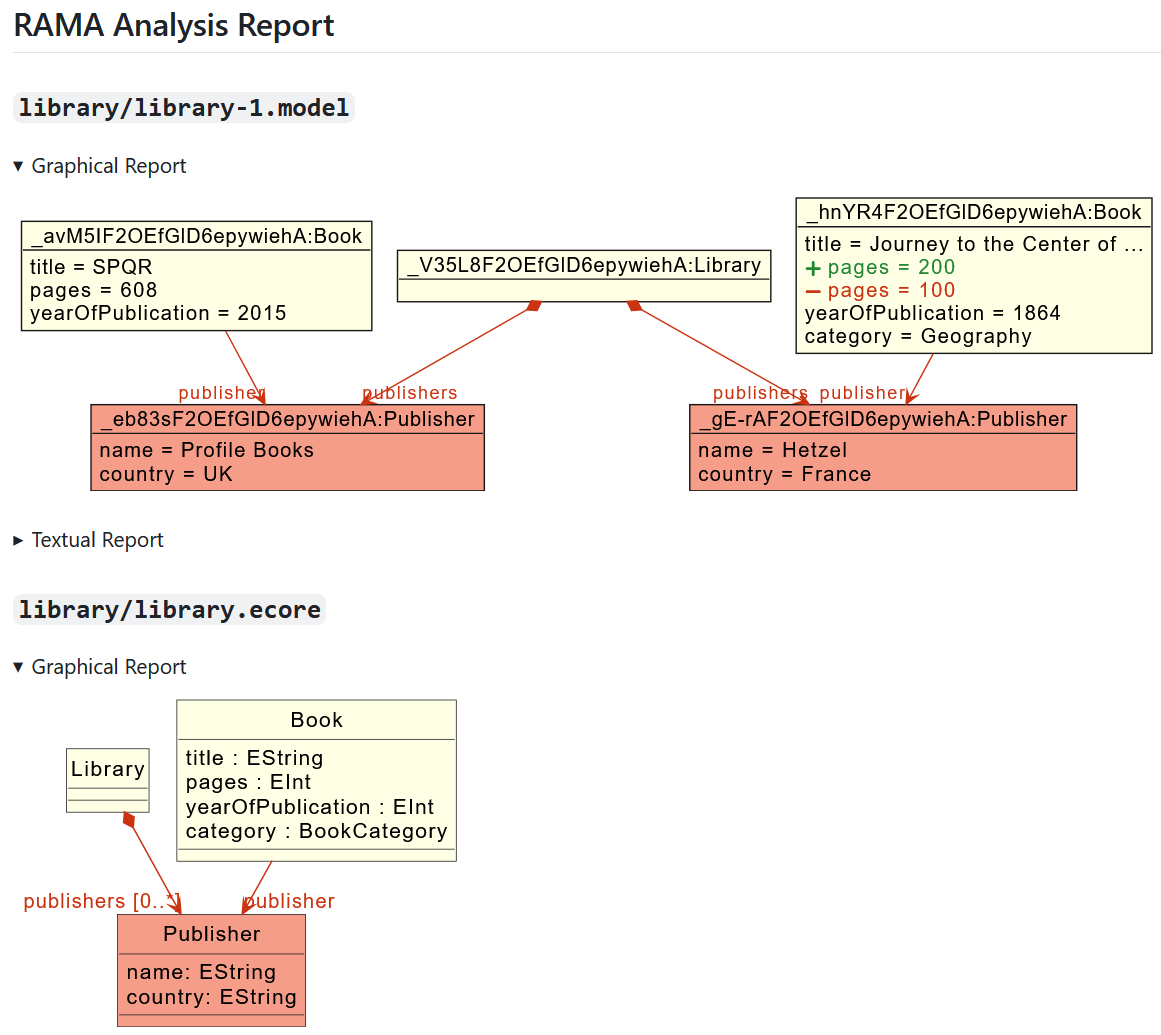
\includegraphics[width=\textwidth]{resources/ejemplo_informe_completo.png}
    \caption{Ejemplo de comentario publicado por RAMA en una \textit{pull request}.}
    \label{fig:informe-generado-ejemplo}
\end{figure}

En el metamodelo, RAMA identifica la eliminación de la clase \texttt{Publisher}, junto con sus atributos y las referencias que la conectaban con \texttt{Library} y \texttt{Book}. En el modelo conforme a ese metamodelo, el informe refleja la desaparición de las instancias \texttt{publisher1} y \texttt{publisher2}, así como de las referencias desde la biblioteca y desde los libros hacia dichas editoriales. De este modo, el comentario no se limita a indicar que los archivos XMI han cambiado, sino que resume qué elementos del dominio han sido suprimidos y qué relaciones del modelo se han visto afectadas.

El desplegable \textit{Textual Report} se corresponde con el resultado textual generado en formato \texttt{UnifiedDiffFormatter}, como se muestra en la Figura~\ref{fig:munidiff-modelo-textual}.

\texttt{GitHubService} publica un comentario nuevo por cada ejecución del \textit{workflow}. Cada actualización de la \textit{pull request}, por ejemplo tras añadir nuevos \textit{commits} a la rama fuente, provoca una nueva ejecución de RAMA y genera un informe independiente. Los comentarios anteriores no se modifican ni se eliminan, sino que permanecen en la conversación de la \textit{pull request} ordenados cronológicamente.

Esta política permite conservar la evolución cronológica del análisis. Cada comentario queda asociado al estado de la \textit{pull request} en el momento en que se ejecutó RAMA, de modo que el revisor puede comparar los resultados producidos por distintas actualizaciones sin perder la información generada en ejecuciones anteriores.

\newpage

\section{Pruebas}
\label{sec:pruebas}

La validación de RAMA se organizó en varios niveles. En primer lugar se añadieron pruebas unitarias sobre las clases con lógica propia y pocas dependencias externas. En segundo lugar se incorporaron pruebas de integración ligeras para comprobar la carga y comparación de modelos EMF reales. Finalmente, para validar el comportamiento completo dentro de GitHub, se planteó una batería de pruebas de sistema basada en repositorios y \textit{pull requests} reales.

\subsection{Pruebas unitarias}

Las pruebas unitarias se ejecutan con JUnit 5 mediante Maven \cite{junit5,maven-surefire}. Su objetivo es comprobar funcionalidad básica de la herramienta sin depender de GitHub ni de repositorios remotos. Estas pruebas se centran en la lectura y procesado del fichero de configuración de RAMA, la generación del contenido del comentario y los servicios auxiliares de renderizado.

\texttt{ConfigServiceTest} valida la carga de la configuración del repositorio. Comprueba que un fichero \texttt{rama.json} ausente, vacío o malformado activa la configuración por defecto y produce una advertencia para el comentario de la \textit{pull request}; también verifica que una configuración válida se aplique sin advertencias.

En \texttt{RamaConfigTest} se comprueba que RAMA identifique correctamente los archivos relevantes según las extensiones configuradas en el fichero \texttt{rama.json}. Estas pruebas cubren archivos de modelo, archivos de metamodelo, extensiones no relevantes, nombres nulos y listas de configuración nulas. También verifican que las rutas de metamodelos se devuelvan de forma segura incluso cuando el campo \texttt{metamodels} no aparece en la configuración.

\texttt{PlantUMLEncoderServiceTest} se encarga de validar la codificación utilizada para generar URLs de PlantUML (ver Sección~\ref{sec:plantuml-encoding}). Se prueban entradas nulas, vacías y en blanco, la construcción de URLs con servidor por defecto, servidores con y sin barra final, y la estabilidad de la codificación mediante una comprobación de ida y vuelta con el decodificador de PlantUML. Esta parte es importante porque el comentario publicado por RAMA no adjunta imágenes, sino URLs que deben poder ser interpretadas por un servidor PlantUML.

En \texttt{ReportCommentRendererTest} se comprueba la estructura del comentario publicado en GitHub. Las pruebas verifican que un informe vacío produzca el mensaje correspondiente, que los archivos se mantengan en orden, que se genere una sección con \texttt{details} e imagen para cada diagrama y que los nombres de archivo y diagnósticos se escapen correctamente para evitar romper el HTML del comentario.

Por último, \texttt{ResourceSafeEcoreMatcherTest} cubre el identificador usado al renderizar diferencias Ecore. Estas pruebas comprueban paquetes, clases, anotaciones, entradas de mapas y objetos Ecore sin recurso asociado. Este punto fue especialmente relevante porque los metamodelos pueden contener elementos sin una URI de recurso directa, y el renderizado debe poder identificarlos sin lanzar excepciones.

\subsection{Pruebas de integración}

Además de las pruebas unitarias, \texttt{EmfModelComparatorTest} ejercita una parte más cercana al comportamiento real de RAMA: la carga de contenido XMI como recursos EMF y la comparación mediante EMF Compare. Estas pruebas no usan GitHub, pero sí utilizan la infraestructura real de EMF, por lo que permiten detectar problemas que no aparecerían en una prueba puramente aislada.

La suite comprueba que dos metamodelos Ecore idénticos produzcan una comparación sin diferencias, que un cambio de nombre en paquete o clase produzca diferencias, y que los contenidos nulos de source, target o base se traten como versiones ausentes sin provocar un fallo. También se prueba que las rutas de metamodelos configuradas se resuelvan de forma relativa al workspace y que, una vez registrado el metamodelo, un modelo conforme pueda cargarse y compararse correctamente.

Estas pruebas de integración cubren la frontera más delicada de la herramienta: el paso desde cadenas de texto recuperadas de GitHub a recursos EMF comparables. Por tanto, complementan las pruebas unitarias y dan confianza en que el núcleo de comparación funciona antes de ejecutar RAMA dentro de un \textit{workflow} real.

\subsection{Pruebas de sistema}

A la hora de realizar las pruebas de sistema, me enfrenté al problema de generar cambios en repositorios de GitHub de forma rápida y en masa. RAMA se ejecuta sobre \textit{pull requests} reales, por lo que no bastaba con tener archivos de ejemplo locales: era necesario crear ramas, \textit{commits} y \textit{pull requests} en GitHub para activar el \textit{workflow} y comprobar el comentario publicado por la herramienta. Para resolver este problema desarrollé un proyecto auxiliar, \texttt{reprogit}, a partir de un script inicial de Alfonso de la Vega Ruiz\footnote{\url{https://github.com/alfonsodelavega/reprogit}}.

El objetivo original de \texttt{reprogit} era generar repositorios Git reproducibles a partir de una colección de carpetas que actúan como \textit{fixtures}. Cada carpeta representa un \textit{commit} y contiene los archivos que deben aparecer modificados en ese punto de la historia. El nombre de la carpeta determina el orden temporal del \textit{commit} y, opcionalmente, la rama en la que debe aplicarse. Por ejemplo, una carpeta asociada a la rama \texttt{add-metamodel} permite crear automáticamente esa rama desde \texttt{main} y añadir en ella los cambios necesarios para probar un caso concreto.

Sin embargo, la generación local del repositorio no era suficiente para validar RAMA en condiciones reales de ejecución. Por este motivo, \texttt{reprogit} se amplió para cubrir también la interacción con GitHub, incluyendo la publicación de ramas y la creación automática de \textit{pull requests}.

Además de crear \textit{commits} y ramas locales, \texttt{reprogit} puede publicar el resultado en un repositorio de GitHub. Para ello usa una configuración con la URL remota del repositorio y un archivo \texttt{.pullrequests.json} donde se describen las \textit{pull requests} que se quieren abrir: título, rama origen, rama destino y descripción. En cada ejecución, el proyecto puede limpiar el repositorio remoto de pruebas, eliminar ramas no principales, cerrar \textit{pull requests} abiertas, forzar la subida de las ramas generadas y crear de nuevo las \textit{pull requests} configuradas.

Esta automatización permite probar RAMA en escenarios repetibles sin preparar manualmente cada repositorio. Se pueden definir casos de prueba para cambios en modelos, cambios en metamodelos, altas y eliminaciones de archivos, modificaciones simultáneas en varios artefactos o situaciones de error. Al ejecutar \texttt{reprogit}, esos casos se convierten en \textit{pull requests} reales sobre GitHub, activando el \textit{workflow} de RAMA y permitiendo comprobar si la herramienta detecta los archivos relevantes, calcula correctamente las diferencias y publica el informe esperado.

La Figura~\ref{fig:reprogit-pull-requests} muestra un ejemplo de las \textit{pull requests} creadas automáticamente por \texttt{reprogit} en el repositorio de pruebas. Cada una representa un escenario reproducible y activa una ejecución independiente de RAMA, lo que permite ejercitar el \textit{workflow} completo sin crear manualmente las ramas, los \textit{commits} ni las revisiones en GitHub.

\begin{figure}[htbp]
    \centering
    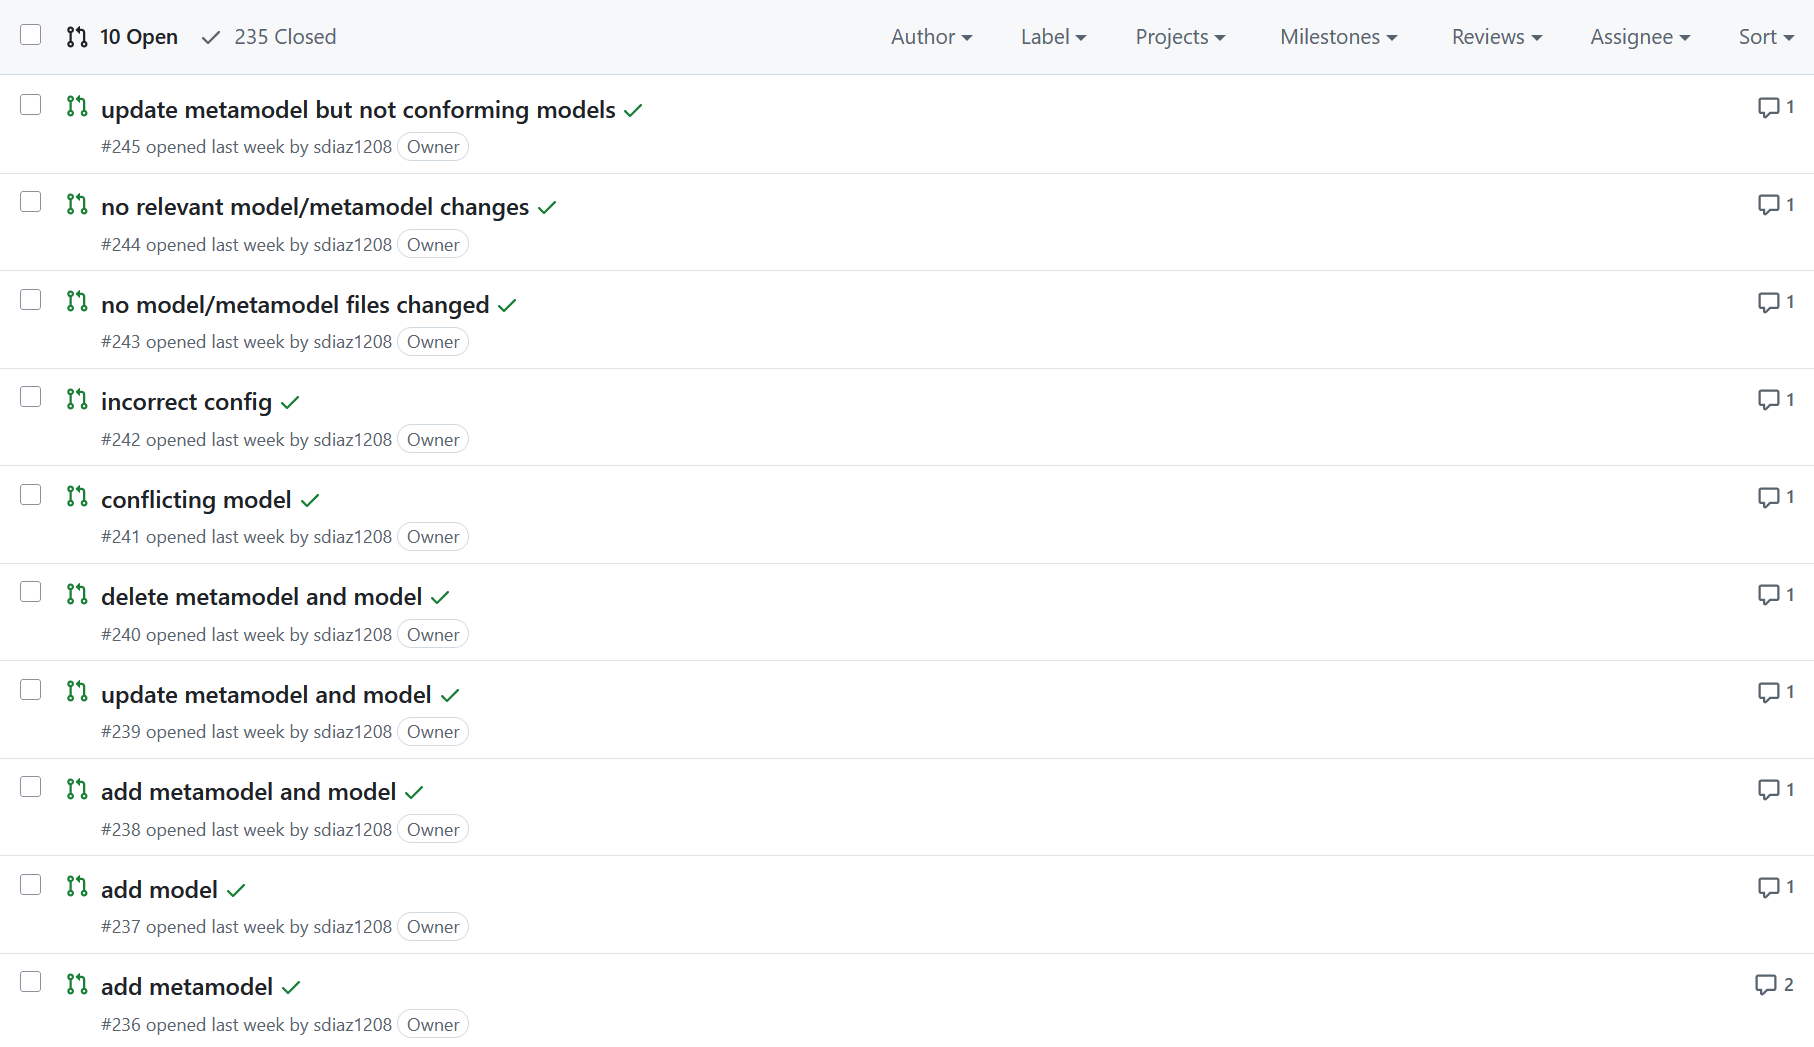
\includegraphics[width=0.9\textwidth]{resources/pull_requests.png}
    \caption{Ejemplo de \textit{pull requests} creadas automáticamente por \texttt{reprogit} para ejecutar pruebas de sistema de RAMA.}
    \label{fig:reprogit-pull-requests}
\end{figure}

Con esta automatización, la preparación y ejecución de las pruebas de sistema queda prácticamente cubierta: \texttt{reprogit} genera los escenarios, y publica las \textit{pull requests}. Con cada publicación de una \textit{pull request}, se activa automáticamente el \textit{workflow} de RAMA. La validación final, sin embargo, sigue requiriendo que una persona revise los informes generados y compruebe que representan correctamente los cambios esperados.

El uso de este proyecto auxiliar también facilitó las pruebas de regresión durante el desarrollo. Cuando se modificaba una parte de RAMA, los mismos \textit{fixtures} podían volver a publicarse sobre el repositorio de pruebas para validar que los comentarios generados seguían siendo coherentes. De esta forma, \texttt{reprogit} convirtió la preparación de repositorios de prueba, ramas y \textit{pull requests} en una tarea automática, rápida y reproducible.

La ampliación de \texttt{reprogit} constituye, por tanto, una contribución adicional de este proyecto. Además de servir como herramienta de apoyo durante el desarrollo, permitió construir un ejemplo específico para las pruebas de sistema de RAMA, con repositorios, ramas y \textit{pull requests} diseñados para ejercitar los casos relevantes de la herramienta. Este ejemplo se puede consultar en el propio repositorio de rama\footnote{\url{https://github.com/sdiaz1208/rama/tree/master/tests/system/fixture}}.

\subsubsection{Casos interesantes}

RAMA presenta varios casos interesantes durante las pruebas de sistema. A continuación se exponen tres de ellos, que ilustran la interacción entre la herramienta y GitHub Actions.

\textbf{Caso 1: actualizando una \textit{pull request} existente}

Para simular dos actualizaciones sucesivas sobre una misma \textit{pull request}, fue necesario incorporar un mecanismo de \textit{polling} en \texttt{reprogit}. Antes de publicar el siguiente \textit{commit}, la herramienta consulta periódicamente el estado de los \textit{workflows} asociados a la revisión y espera a que termine la ejecución en curso. Esta solución es deliberadamente sencilla, pero evita que GitHub Actions procese ambos cambios como si fueran simultáneos: en ese caso, las dos ejecuciones de RAMA podían analizar el mismo estado final de la rama y publicar dos informes idénticos. Con la espera, cada \textit{commit} activa una ejecución que analiza el estado que le corresponde.

\textbf{Caso 2: modificando un metamodelo sin modificar los modelos conformes}

Otra limitación aparece cuando una \textit{pull request} modifica un metamodelo sin modificar los modelos que se ajustan a él. RAMA determina los artefactos que debe analizar a partir de los ficheros modificados en la revisión, por lo que no identifica ni valida posibles incompatibilidades en modelos que no figuran entre dichos cambios. Esta comprobación se considera fuera del ámbito de RAMA: la herramienta está orientada a enriquecer la revisión de los cambios presentes en una \textit{pull request}, no a actuar como un sistema de integración continua encargado de validar globalmente la conformidad de todos los modelos del repositorio tras cada modificación del metamodelo.

\textbf{Caso 3: añadiendo un metamodelo y un modelo conforme en la misma \textit{pull request}}

También aparece una limitación cuando una misma \textit{pull request} añade un modelo y el metamodelo Ecore del que depende. RAMA recupera mediante la API de GitHub el contenido del modelo desde la rama fuente, pero carga los metamodelos configurados desde el \textit{workspace} local. El \textit{workflow} se ejecuta con el evento \texttt{pull\_request\_target}, por lo que dicho \textit{workspace} contiene la rama destino y todavía no incluye el metamodelo recién añadido. En consecuencia, EMF no puede resolver el metamodelo al cargar el modelo, y la comparación no se completa aunque ambos archivos formen parte de la revisión.

Resolver este caso requiere que RAMA obtenga también los metamodelos configurados desde la rama que se está analizando, en lugar de depender únicamente de los disponibles en la rama destino. Esta mejora se deja como trabajo futuro, ya que exige revisar el mecanismo de carga de metamodelos.

\newpage

\section{Conclusiones y Trabajo Futuro}
\label{sec:conclusiones-trabajo-futuro}

RAMA introduce información a nivel de modelo en el proceso habitual de revisión de las \textit{pull requests}. Su principal aportación es desplazar la revisión desde el texto serializado hacia los elementos reales del modelo: elementos añadidos, eliminados, atributos modificados y referencias actualizadas. Esto reduce ruido y facilita la comprensión de cambios en proyectos basados en Ingeniería del software Dirigida por Modelos.

El trabajo realizado demuestra que es posible integrar comparación de modelos en una plataforma de revisión generalista sin modificar el flujo de trabajo del desarrollador. GitHub sigue actuando como punto de entrada de la revisión y como medio de publicación del resultado, mientras que RAMA añade una capa de análisis específica para artefactos EMF.

Como trabajo futuro, se plantean varias líneas de mejora:

\begin{itemize}
    \item Ampliar la configuración de \texttt{rama.json} con reglas de inclusión y exclusión de rutas, de forma que cada repositorio pueda limitar el análisis a carpetas concretas o excluir artefactos generados.
    \item Añadir validación explícita de la configuración de RAMA, incluyendo errores y advertencias que puedan aparecer en el informe de la \textit{pull request}.
    \item Enriquecer los resultados del análisis para distinguir de forma estructurada entre cambios sintácticos, ausencia de cambios de modelo, fallos de carga, problemas de metamodelo y análisis incompletos.
    \item Incorporar detección específica de cambios textuales que no produzcan cambios reales en el modelo cargado, para informar al revisor cuando una modificación sea solo ruido de serialización.
    \item Implementar un modo local o de depuración que permita ejecutar RAMA sobre \textit{fixtures} o directorios locales sin depender de una \textit{pull request} real ni publicar comentarios.
    \item Adaptar la carga de metamodelos configurados para obtenerlos desde la rama de la \textit{pull request} analizada. De este modo, RAMA podría comparar modelos y metamodelos añadidos conjuntamente en una revisión, sin depender de que dichos metamodelos ya existan en el \textit{workspace} de la rama destino cuando se usa \texttt{pull\_request\_target}.
    \item Permitir configurar servidores personales y privados para el renderizado de los informes gráficos. Esto evitaría enviar a servidores públicos descripciones PlantUML derivadas de modelos que puedan contener información sensible o propiedad intelectual del proyecto.
    \item Automatizar la validación de los informes generados en las pruebas de sistema. Actualmente esta fase requiere revisión manual; una posible línea sería definir oráculos para comparar automáticamente los informes obtenidos con salidas esperadas, aunque este enfoque también introduce inconvenientes, como el coste de mantener dichos oráculos y su sensibilidad ante cambios legítimos en el formato del informe.
    \item Explorar la adaptación de la arquitectura a otros proveedores de control de versiones como GitLab o Bitbucket.
    \item Permitir el uso de metamodelos proporcionados como dependencias externas, no necesariamente incluidos en el repositorio analizado, como por ejemplo ocurre en proyectos que utilizan modelos UML o BPMN basados en EMF.
    \item Incorporar soporte por defecto para formatos habituales en herramientas de modelado del ecosistema EMF, como modelos Flexmi (\texttt{.flexmi}) \cite{Flexmi} o metamodelos Emfatic (\texttt{.emf}) \cite{emfatic}.
    \item Evaluar RAMA con desarrolladores que trabajen habitualmente con MDSE, con el objetivo de recoger \textit{feedback} sobre su utilidad, la claridad de los informes generados y posibles mejoras en el flujo de revisión.
\end{itemize}

\newpage

\addcontentsline{toc}{section}{Referencias}

\begin{thebibliography}{99}

\bibitem{progit}
Scott Chacon y Ben Straub.
\textit{Pro Git}.
Apress, 2.\textsuperscript{a} edición, 2014.
\url{https://git-scm.com/book/en/v2}

\bibitem{tortoisegitmerge-conflicts}
TortoiseGit contributors.
\textit{TortoiseGitMerge Manual: Editing Conflicts}.
\url{https://tortoisegit.org/docs/tortoisegitmerge/tmerge-basics-conflicts.html}

\bibitem{brambilla-mdse}
Marco Brambilla, Jordi Cabot y Manuel Wimmer.
\textit{Model-Driven Software Engineering in Practice}.
Morgan \& Claypool, 2012.

\bibitem{autosar}
AUTOSAR.
\textit{AUTOSAR: The standardized software framework for intelligent mobility}.
\url{https://www.autosar.org/}

\bibitem{ieee-aerospace-mdse}
IEEE Xplore.
\textit{Document 9592422}.
\url{https://ieeexplore.ieee.org/document/9592422}

\bibitem{mbeddr}
mbeddr project.
\textit{mbeddr: Engineering the Future of Embedded Software Development}.
\url{https://mbeddr.com/}

\bibitem{outsystems}
OutSystems.
\textit{Low-Code Application Development Platform}.
\url{https://www.outsystems.com/low-code/}

\bibitem{emf-book}
Dave Steinberg, Frank Budinsky, Marcelo Paternostro y Ed Merks.
\textit{EMF: Eclipse Modeling Framework}.
Addison-Wesley Professional, 2.\textsuperscript{a} edición, 2008.

\bibitem{emf-docs}
Eclipse Foundation.
\textit{The Eclipse Modeling Framework (EMF) Overview}.
\url{https://help.eclipse.org/latest/topic/org.eclipse.emf.doc/references/overview/EMF.html}

\bibitem{XMI}
Object Management Group.
\textit{XML Metadata Interchange (XMI) Specification}.
Junio de 2015.
\url{https://www.omg.org/spec/XMI/About-XMI/}

\bibitem{Flexmi}
Dimitris Kolovos y Alfonso de la Vega.
``Flexmi: a generic and modular textual syntax for domain-specific modelling''.
\textit{Software and Systems Modeling}, 2022.
\url{https://doi.org/10.1007/s10270-022-01064-3}

\bibitem{emfatic}
Eclipse Foundation.
\textit{Emfatic}.
\url{https://eclipse.dev/emfatic/}

\bibitem{sirius-docs}
Eclipse Foundation.
\textit{Eclipse Sirius Documentation}.
\url{https://eclipse.dev/sirius/doc/}

\bibitem{epsilon-docs}
Eclipse Foundation.
\textit{Eclipse Epsilon Documentation}.
\url{https://eclipse.dev/epsilon/doc/}

\bibitem{emfcompare-overview}
Eclipse Foundation.
\textit{EMF Compare Overview}.
\url{https://eclipse.dev/emfcompare/overview.html}

\bibitem{emfcompare-api}
Eclipse Foundation.
\textit{EMF Compare API Specification}.
\url{https://help.eclipse.org/latest/topic/org.eclipse.emf.compare.doc/help/developer/javadoc/org/eclipse/emf/compare/EMFCompare.html}

\bibitem{delavega-thesis}
Alfonso de la Vega.
\textit{Domain-Specific Languages for Data Mining Democratisation}.
Tesis doctoral, Universidad de Cantabria, 2019.
\url{http://hdl.handle.net/10902/16728}

\bibitem{flandm}
Alfonso de la Vega, Diego García-Saiz, Marta E. Zorrilla y Pablo Sánchez.
``FLANDM: a development framework of domain-specific languages for data mining democratisation''.
\textit{Computer Languages, Systems \& Structures}, 54:316--336, 2018.
\url{https://doi.org/10.1016/j.cl.2018.07.002}

\bibitem{model-driven-data-mining}
Alfonso de la Vega y Pablo Sánchez.
``Model-Driven Technologies for Data Mining Democratisation''.
\textit{Software Technologies: Applications and Foundations, Junior Researchers Community Event}, CEUR Workshop Proceedings, Vol. 2405, pp. 9--14, 2019.
\url{https://ceur-ws.org/Vol-2405/03_paper.pdf}

\bibitem{lavoisier}
Alfonso de la Vega, Diego García-Saiz, Marta E. Zorrilla y Pablo Sánchez.
``Lavoisier: A DSL for increasing the level of abstraction of data selection and formatting in data mining''.
\textit{Journal of Computer Languages}, 60:100987, 2020.
\url{https://doi.org/10.1016/j.cola.2020.100987}

\bibitem{pinset}
Alfonso de la Vega, Pablo Sánchez y Dimitrios S. Kolovos.
``Pinset: A DSL for extracting datasets from models for data mining-based quality analysis''.
\textit{Proceedings of the 2018 International Conference on the Quality of Information and Communications Technology (QUATIC)}, pp. 83--91, IEEE, 2018.
\url{https://doi.org/10.1109/QUATIC.2018.00021}

\bibitem{peacemaker}
Alfonso de la Vega y Dimitris Kolovos.
``An efficient line-based approach for resolving merge conflicts in XMI-based models''.
\textit{Software and Systems Modeling}, 21(6):2461--2487, 2022.
\url{https://doi.org/10.1007/s10270-022-00976-4}

\bibitem{picto}
Eclipse Foundation.
\textit{Visualising Models with Picto}.
\url{https://eclipse.dev/epsilon/doc/picto/}

\bibitem{picto-diff}
Epsilon Labs.
\textit{Picto Diff}.
\url{https://github.com/epsilonlabs/picto-diff}

\bibitem{munidiff}
Munidiff project.
\textit{Munidiff timeline client}.
\url{https://github.com/munidiff/munidiff.github.io}

\bibitem{munidiff-paper}
Alfonso de la Vega.
``Towards an Interoperable Textual Format for Model Differences Reporting''.
\textit{2023 ACM/IEEE International Conference on Model Driven Engineering Languages and Systems Companion (MODELS-C)}, pp. 924--928, 2023.
\url{https://dblp.org/rec/conf/models/Vega23}

\bibitem{timeline-paper}
Alfonso de la Vega.
``Timeline exploration of model differences in source code repositories through graphical and textual views''.
\textit{Proceedings of the ACM/IEEE 27th International Conference on Model Driven Engineering Languages and Systems (MODELS Companion '24)}, pp. 755--759, ACM, 2024.
\url{https://doi.org/10.1145/3652620.3688207}

\bibitem{plantuml}
PlantUML project.
\textit{PlantUML Documentation}.
\url{https://plantuml.com/}

\bibitem{plantuml-server}
PlantUML project.
\textit{PlantUML Server}.
\url{https://plantuml.com/es/server}

\bibitem{kroki}
Kroki project.
\textit{Kroki}.
\url{https://kroki.io/}

\bibitem{github-actions}
GitHub.
\textit{GitHub Actions Documentation}.
\url{https://docs.github.com/en/actions}

\bibitem{junit5}
JUnit Team.
\textit{JUnit 5 User Guide}.
\url{https://junit.org/junit5/docs/current/user-guide/}

\bibitem{maven-surefire}
Apache Maven Project.
\textit{Maven Surefire Plugin}.
\url{https://maven.apache.org/surefire/maven-surefire-plugin/}

\end{thebibliography}

\newpage

\appendix

\section{Ejemplo de \textit{Workflow} de GitHub Actions}
\label{app:workflow-github-actions}

El siguiente es un ejemplo de archivo \texttt{rama.yml} que se puede incluir en el directorio \texttt{.github/workflows} de un repositorio para ejecutar RAMA automáticamente en cada una de las \textit{pull requests} \cite{github-actions}, siendo este \textit{workflow} válido en el momento en que esta memoria se ha escrito (la herramienta seguirá evolucionando en el tiempo):

\begin{lstlisting}[caption={Ejemplo de \textit{Workflow} de GitHub Actions.},label={lst:workflow-github-actions}]
name: RAMA Analysis

# Ejecuta RAMA cuando se crea, actualiza o reabre una pull request.
on:
  pull_request_target:
    types: [opened, synchronize, reopened]

# Permisos minimos: leer el repositorio y escribir comentarios en la PR.
permissions:
  contents: read
  pull-requests: write

jobs:
  analyze:
    # Maquina virtual donde se ejecuta el analisis.
    runs-on: ubuntu-latest

    steps:
      # Descarga el repositorio que contiene la pull request.
      - name: Checkout PR repo
        uses: actions/checkout@v4

      # Clona el repositorio de RAMA para compilar y ejecutar la herramienta.
      - name: Clone RAMA
        run: git clone --branch feature/vertical-slice --single-branch https://github.com/sdiaz1208/rama.git

      # Instala Java 21 y activa cache de dependencias Maven.
      - name: Setup Java
        uses: actions/setup-java@v4
        with:
          distribution: temurin
          java-version: 21
          cache: maven
          cache-dependency-path: rama/pom.xml

      # Instala EMF Compare en el repositorio local de Maven.
      - name: Install EMF Compare locally
        run: |
          mvn install:install-file \
            -Dfile=libs/org.eclipse.emf.compare_3.5.3.202406060900.jar \
            -DgroupId=org.eclipse.emf.compare \
            -DartifactId=org.eclipse.emf.compare \
            -Dversion=3.5.3 \
            -Dpackaging=jar
        working-directory: rama

      # Instala las librerias de Modiff necesarias para generar informes.
      - name: Install Modiff libs locally
        run: |
          mvn install:install-file \
            -Dfile=libs/org.eclipse.epsilon.modiff-0.0.1-SNAPSHOT.jar \
            -DpomFile=libs/org.eclipse.epsilon.modiff-0.0.1-SNAPSHOT.pom.xml

          mvn install:install-file \
            -Dfile=libs/org.eclipse.epsilon.modiff.emfcompare-0.0.1-SNAPSHOT.jar \
            -DpomFile=libs/org.eclipse.epsilon.modiff.emfcompare-0.0.1-SNAPSHOT.pom.xml
        working-directory: rama

      # Compila RAMA y genera el JAR ejecutable.
      - name: Build RAMA
        run: mvn clean package
        working-directory: rama

      # Ejecuta RAMA sobre la pull request que disparo el workflow.
      - name: Run RAMA
        run: java -jar target/RAMA.jar ${{ github.event.pull_request.number }}
        working-directory: rama
        env:
          # Token usado para consultar la PR y publicar el comentario.
          GITHUB_TOKEN: ${{ secrets.GITHUB_TOKEN }}
          # Repositorio sobre el que se esta ejecutando el workflow.
          GITHUB_REPOSITORY: ${{ github.repository }}
\end{lstlisting}

\newpage

\section{Manual de Usuario y Desarrollador}
\label{app:manual-usuario-desarrollador}

Este apéndice resume los pasos necesarios para utilizar RAMA en un repositorio de GitHub y las tareas básicas para continuar su desarrollo. El manual se divide en dos partes: una orientada al usuario que quiere activar la herramienta en su proyecto, y otra orientada al desarrollador que quiere compilar, probar o modificar RAMA.

\subsection{Uso de RAMA en un repositorio}

Para utilizar RAMA en un repositorio de GitHub es necesario añadir un \textit{workflow} de GitHub Actions similar al mostrado en el Apéndice~\ref{app:workflow-github-actions} \cite{github-actions}. Este \textit{workflow} debe ejecutarse cuando se abra, actualice o reabra una \textit{pull request}. La acción compila RAMA, ejecuta el archivo \texttt{RAMA.jar} y le pasa como argumento el número de la \textit{pull request} que se está analizando.

El repositorio donde se instala RAMA debe cumplir las siguientes condiciones:

\begin{itemize}
    \item Tener activadas las acciones de GitHub.
    \item Permitir al \textit{workflow} leer el contenido del repositorio y escribir comentarios en las \textit{pull requests}.
    \item Contener los modelos y metamodelos que se quieren analizar.
    \item Incluir un archivo \texttt{rama.json} si se necesita una configuración distinta a la configuración por defecto.
\end{itemize}

La configuración se coloca en la raíz del repositorio mediante el archivo \texttt{rama.json}. En él se indican las extensiones que RAMA debe considerar modelos, las extensiones que debe considerar metamodelos y, opcionalmente, las rutas de los metamodelos que deben registrarse antes de cargar los modelos. Por ejemplo, un proyecto que utiliza modelos \texttt{.model} y metamodelos \texttt{.ecore} puede usar la configuración del Listado~\ref{lst:rama-config}.

Cuando se crea una \textit{pull request}, RAMA recupera la lista de archivos modificados y selecciona aquellos cuya extensión aparece en la configuración. Para cada archivo relevante obtiene tres versiones: la versión de la rama fuente, la versión de la rama objetivo y la versión del \textit{merge-base}. Después compara esas versiones con EMF Compare y publica un comentario en la \textit{pull request}.

\subsection{Interpretación del informe}

El informe generado por RAMA aparece como un comentario automático en la \textit{pull request}. El comentario contiene una sección por cada modelo o metamodelo analizado. Cuando EMF Compare detecta diferencias, la sección muestra un bloque desplegable con el reporte gráfico y, en el caso de los modelos, otro con el reporte textual. Si no hay diferencias a nivel de modelo, RAMA muestra un mensaje informativo en lugar de los desplegables; para una eliminación sin renombre informa que el archivo se ha eliminado. Cuando EMF Compare detecta conflictos, la sección presenta dos vistas gráficas de los cambios de las ramas fuente y objetivo respecto al \textit{merge-base}. En los informes gráficos y textuales, los elementos añadidos se resaltan en verde y los eliminados en rojo.

Si un modelo o metamodelo no puede analizarse por culpa de algún error, RAMA mantiene la sección correspondiente e incluye un diagnóstico breve. Este diagnóstico indica el tipo de fallo y remite a los logs de GitHub Actions para consultar la traza completa. De este modo, un error en un modelo o metamodelo concreto no impide obtener información sobre los demás archivos de la \textit{pull request}.

Si el autor de la \textit{pull request} sube nuevos \textit{commits}, el \textit{workflow} vuelve a ejecutar RAMA y la herramienta publica un comentario nuevo con el resultado de esa actualización. Los comentarios anteriores permanecen en la conversación, de forma que el revisor puede consultar el historial completo de análisis en orden cronológico.

\subsection{Problemas frecuentes de uso}

Los problemas más habituales al utilizar RAMA están relacionados con la configuración o con la carga de modelos:

\begin{itemize}
    \item Si no aparece ningún archivo en el informe, conviene revisar que las extensiones de \texttt{rama.json} coincidan con los archivos modificados.
    \item Si un modelo no carga, debe comprobarse que su metamodelo esté disponible en el repositorio y que su ruta figure en el campo \texttt{metamodels}.
    \item Si el \textit{workflow} no puede publicar comentarios, hay que revisar los permisos de GitHub Actions, especialmente el permiso \texttt{pull-requests: write}.
    \item Si el archivo \texttt{rama.json} no existe, está vacío o contiene JSON inválido, RAMA utiliza la configuración por defecto e incluye una advertencia de configuración en el comentario de la \textit{pull request}.
\end{itemize}

\subsection{Desarrollo local}

El código fuente de RAMA se encuentra disponible en el siguiente repositorio público: \url{https://github.com/sdiaz1208/rama}.

Para desarrollar RAMA localmente se necesita Java 21 y Maven. El código fuente se organiza en paquetes separados para configuración, integración con GitHub, comparación de modelos, renderizado e inicialización de la aplicación.

Las tareas básicas de desarrollo son:

\begin{itemize}
    \item Compilar el proyecto con \texttt{mvn clean package}.
    \item Ejecutar las pruebas con \texttt{mvn test}.
    \item Revisar la configuración por defecto en \texttt{rama.json}.
    \item Consultar el \textit{workflow} de ejemplo en \texttt{rama.yml}.
    \item Modificar o añadir pruebas en \texttt{src/test/java} cuando se cambie comportamiento de la herramienta.
\end{itemize}

El punto de entrada de la aplicación es \texttt{Main}. Esta clase carga la configuración, crea las dependencias principales y delega la ejecución en \texttt{RamaApplication}. La lógica de comunicación con GitHub se encuentra detrás de la interfaz \texttt{GitService}; la comparación de modelos se encuentra detrás de \texttt{ComparisonService}; y la generación del informe se concentra en \texttt{MunidiffRenderer}, \texttt{PlantUMLEncoderService} y \texttt{ReportCommentRenderer}.

Esta separación facilita añadir nuevas pruebas o sustituir componentes concretos. Por ejemplo, un proveedor distinto de GitHub podría implementarse creando una nueva clase que implemente \texttt{GitService}, mientras que un mecanismo de comparación alternativo podría integrarse implementando \texttt{ComparisonService}.

\subsection{Pruebas durante el desarrollo}

Antes de publicar cambios en RAMA conviene ejecutar la batería de pruebas automatizadas:

\begin{verbatim}
mvn test
\end{verbatim}

Estas pruebas cubren la configuración, la codificación de URLs PlantUML, la generación del comentario, el identificador de elementos Ecore y la comparación de modelos mediante EMF Compare. Para validar el comportamiento completo en GitHub, se recomienda complementar estas pruebas con casos de sistema que creen ramas, \textit{commits} y \textit{pull requests} reales sobre un repositorio de pruebas. Para ello, se puede usar el proyecto auxiliar \texttt{reprogit}, que automatiza la creación de repositorios reproducibles a partir de \textit{fixtures} locales. Al ejecutar \texttt{reprogit}, se generan las \textit{pull requests} necesarias para activar el \textit{workflow} de RAMA y comprobar que los comentarios publicados contienen la información esperada.

\newpage

\end{document}
